\documentclass[12pt,a4paper]{article}
\usepackage[utf8]{inputenc}
\usepackage[T1]{fontenc}
\usepackage{amsmath}
\usepackage{amsfonts}
\usepackage{amssymb}
\usepackage{graphicx}
\usepackage{geometry}
\usepackage{mathtools}
%\usepackage{diagrams}
\usepackage[document]{ragged2e}
\usepackage{wasysym}
\usepackage{pgfplots}
\usepackage{ mathrsfs }
\usepackage{braket}
\usepackage{simpler-wick}
\usepackage{tikz}
\usetikzlibrary{decorations.markings}
\usepackage{tikz-feynman}
\usepackage{subcaption}
\usepackage{bm}
\usepackage{slashed}
\usepackage{tensor}
\usepackage{hyperref}
\usepackage{float}
\usetikzlibrary{calc}
\tikzset{
	myarrow/.style={stealth-,shorten >=3pt,shorten <=3pt}
}
\pgfplotsset{
	lineplot/.style={
		black,
		dashed,
		very thin,
		samples y=0
	},
	coordinate line/.style={
		black,
		samples y=0
	},
	point/.style={
		only marks,
		mark=*,
		black,
		mark size=0.5pt
	}
}
\title{Topics in Mathematical Physics}
\author{Ben Karsberg}
\date{2021-22}
\newgeometry{vmargin={15mm}, hmargin={20mm,20mm}}
\numberwithin{equation}{section}
\DeclareMathSymbol{:}{\mathord}{operators}{"3A}
\begin{document}
	\maketitle
	\section{Preface}
	\begin{itemize}
		\item These notes were written up for the postgraduate masters course in mathematical physics at the University of Edinburgh
		\item The topic this year was 'Applications of Geometry in Physics'
		\item It was lectured by James Lucietti, who's notes are unfortunately only available on the Edinburgh intranet
		\item These notes were largely produced with those official notes as reference
		\item These notes were written primarily with myself in mind; it has some colloquialisms in it, and some topics are presented in the way I best understand them, and not necessarily the `best' way
		\item The notes are also exclusively bullet pointed because I find prose difficult to digest
		\item Any errors are most certainly mine and not James's - let me know at \href{mailto:benkarsberg@gmail.com}{benkarsberg@gmail.com} if you note any bad ones
		\item Generally, text in \textit{italic} is the definition of something the first time it shows up, and text in \textbf{bold} is something I think is important/want to remember/found tricky when writing these up
		\item Summation convention is implicit throughout this entire set of notes, unless explicitly stated otherwise
		\item Euclidean spatial vectors are denoted by e.g. $\mathbf{v}$, and 4-vectors are denoted by just $v=(v^{0},\mathbf{v})$
		\item The metric signature is $\eta_{\mu\nu}=\text{diag}(+1,-1,-1,-1)$ unless stated otherwise
		\item $\hbar=c=1$
		\item I hope these notes are helpful to someone who isn't me - enjoy!
	\end{itemize}
	\newpage
	\section{Differential Geometry Preliminaries}
	\begin{itemize}
		\item This course is all about geometry, almost entirely differential
		\item Differentiable geometry is a listed prerequisite for this course, but I haven't done any properly, with the exception of pseudo-Riemannian geometry in coordinate bases in a GR course last year
		\item Therefore, we need to set the scene
		\item The principal arena for differential geometry is a \textbf{differential manifold}:
		\begin{itemize}
			\item Informally, this is a set $M$ that locally looks like $\mathbb{R}^{n}$
			\item Formally, this is a topological space $M$ equipped with a collection of charts $\{(U_{\alpha},\phi_{\alpha})\}$ called an \textbf{atlas}, where $\{U_{\alpha}\}$ is an open cover of $M$ and $\phi_{\alpha}\;:\;U_{\alpha}\to V_{\alpha}\subset\mathbb{R}^{n}$ are homeomorphisms
		\end{itemize}
		\item The image we want in mind is something like this, generalised to $\mathbb{R}^{n}$ rather than just $\mathbb{R}^{2}$:
		\begin{figure}[H]
			\centering
		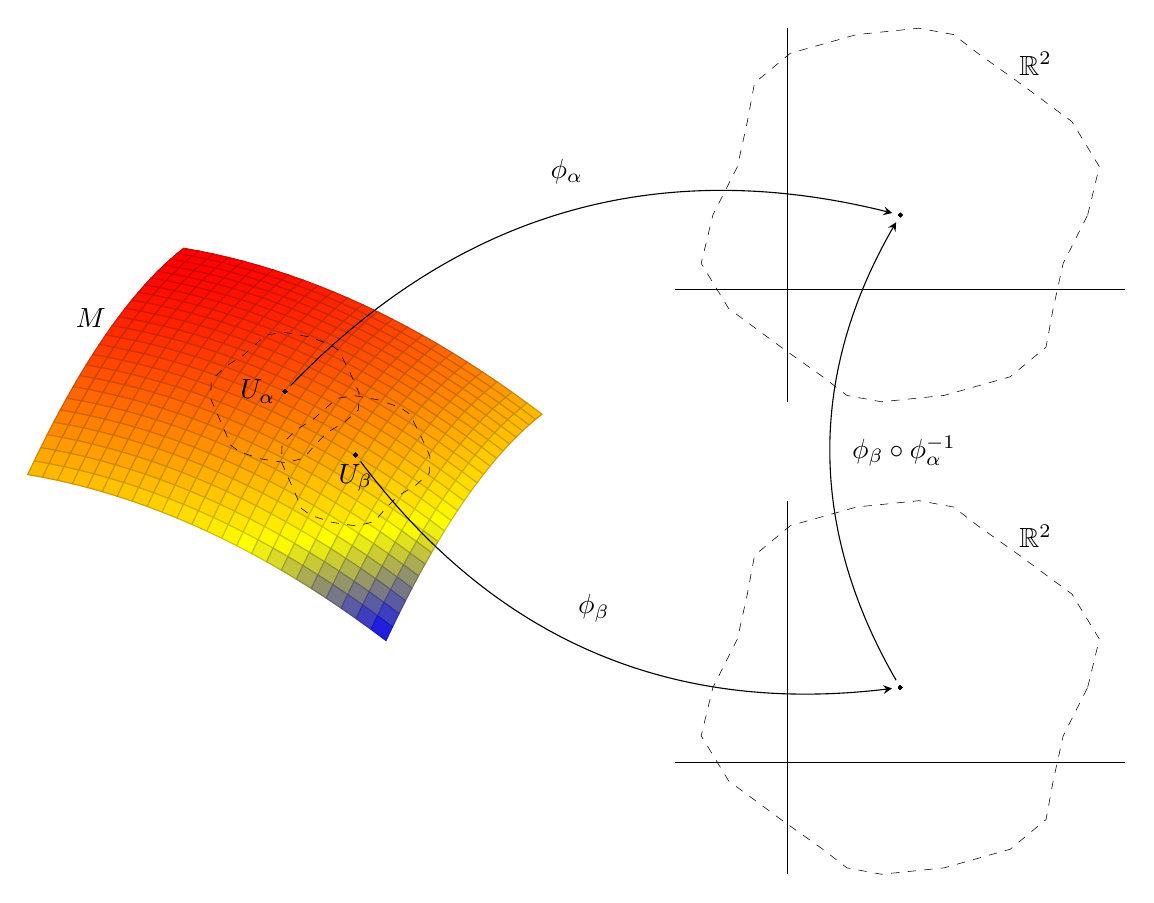
\begin{tikzpicture}
			\begin{axis}[
				name=mfd,
				axis lines=none,
				declare function={
					f(\x,\y)=10-(\x^2+\y^2);
				},
				declare function={
					c_x(\t)=(cos(\t)+(sin(5*\t)/10))/3+1;
				},
				declare function={
					c_y(\t)=(sin(\t))/2-1;
				},
				declare function={
					c_z(\t)=f(c_x(\t),c_y(\t));
				},
				declare function={
					x_0(\t)=-1.2;
				},
				declare function={
					x_1(\t)=0.8;
				}
				]
				\addplot3[surf,domain=0:2,domain y=-2:0,]{f(x,y)};
				\addplot3[lineplot,variable=t,domain=0:360] ({c_x(t)},{c_y(t)},{c_z(t)});
				\addplot3[lineplot,variable=t,domain=0:360] ({c_x(t)+0.7},{c_y(t)-0.7},{c_z(t)});
				%\addplot3[coordinate line,variable=t,domain=0:2] (t,{x_0(t)},{f(t,{x_0(t)})});
				%\addplot3[coordinate line,variable=t,domain=-2:0] ({x_1(t)},t,{f({x_1(t)},t)});
				\addplot3[point] (1,-1,{f(1,-1)}) coordinate (a);
				\addplot3[point] (1.7,-1.7,{f(1,-1)}) coordinate (c);
				%\addplot3[point](.5,{x_0(.5)},{f(.5,{x_0(.5)})}) coordinate (x_dot);
				%\addplot3[point]({x_1(-.5)},-.5,{f({x_1(-.5)},-.5)}) coordinate (y_dot);
			\end{axis}
				\draw (a) node [left] {$U_{\alpha}$};
				\draw (c) node [below] {$U_{\beta}$};
			\begin{axis}[
				at={($(mfd.north east)+(1cm,3cm)$)},
				anchor=north west,
				axis lines=none,
				declare function={
					c_x(\t)=(cos(\t)+(sin(5*\t)/10))/3+1;
				},
				declare function={
					c_y(\t)=(sin(\t))/2-1;
				},
				declare function={
					x_0(\t)=-1.2;
				},
				declare function={
					x_1(\t)=0.8;
				}
				]
				\addplot[lineplot,variable=t,domain=0:360]({c_x(t)},{c_y(t)});
				\addplot[point] (1,-1) coordinate (b);
				\addplot[coordinate line,variable=t,domain=0.6:1.4](t,{x_0(t)});
				\addplot[coordinate line,variable=t,domain=-1.5:-0.5]({x_1(t)},t);
				%\addplot[point](.8,-.5) coordinate (P1);
				%\addplot[point](.6,-1.2) coordinate (P2);
			\end{axis}
			\draw [myarrow] (b) to[bend right] node [above=7pt] {$\phi_{\alpha}$} (a);
			\draw (13,7.5) node [above] {$\mathbb{R}^{2}$};
			\draw (13,1.5) node [above] {$\mathbb{R}^{2}$};
			\draw (1,4.3) node [above] {$M$};
			%\draw [myarrow] (P1) to[bend left] ++(-1cm,1cm) node[above] {$(x \circ \gamma_{(1)})$};
			%\draw [myarrow] (P2) to[bend left] ++(-3cm,-1cm) node[above] {$(x \circ \gamma_{(0)})$};
			\begin{axis}[
				at={($(mfd.north east)+(1cm,-3cm)$)},
				anchor=north west,
				axis lines=none,
				declare function={
					c_x(\t)=(cos(\t)+(sin(5*\t)/10))/3+1;
				},
				declare function={
					c_y(\t)=(sin(\t))/2-1;
				},
				declare function={
					x_0(\t)=-1.2;
				},
				declare function={
					x_1(\t)=0.8;
				}
				]
				\addplot[lineplot,variable=t,domain=0:360]({c_x(t)},{c_y(t)});
				\addplot[point] (1,-1) coordinate (d);
				\addplot[coordinate line,variable=t,domain=0.6:1.4](t,{x_0(t)});
				\addplot[coordinate line,variable=t,domain=-1.5:-0.5]({x_1(t)},t);
			\end{axis}
			\draw [myarrow] (d) to[bend left] node [above=7pt] {$\phi_{\beta}$} (c);
			\draw [myarrow] (b) to[bend right] node [right=4pt] {$\phi_{\beta}\circ\phi_{\alpha}^{-1}$} (d);
		\end{tikzpicture}
		\end{figure}
		\item Essentially, a chart $(U,\phi)$ assigns coordinates to a point $p\in U$ given by $\phi(p)=(x^{1}(p),\ldots,x^{n}(p))$, usually written $\phi=\left(x^{i}\right)$
		\item Importantly, the \textbf{transition functions} $\phi_{\beta}\circ\phi_{\alpha}^{-1}\;:\;\phi_{\beta}(U_{\alpha}\cap U_{\beta})\to\phi_{\alpha}(U_{\alpha}\cap U_{\beta})$ should be $C^{\infty}(\mathbb{R}^{n})$ bijections between open subsets of $\mathbb{R}^{n}$ (see diagram)
		\item Essentially, all changes of coordinates are given by a smooth map
		\item The atlas allows us to define calculus on a manifold, and we can classify a hierarchy of objects on $M$:
		\begin{itemize}
			\item $C^{\infty}(M)$ is the set of all smooth functions on $M$, with the function of a standard commutative algebra
			\item The \textbf{tangent space} $T_{p}M$ at $p\in M$ is the $n$-dimensional vector space of directional derivatives at $p$; that is, the space of all $\mathbb{R}$-linear maps $X_{p}\;:\; C^{\infty}(M)\to\mathbb{R}$ obeying the Leibnitz/product rule
			\begin{equation}
				X_{p}(fg)=X_{p}(f)g(p)+f(p)X_{p}(g)
			\end{equation}
			for all $f,g\in C^{\infty}(M)$
			\item The elements $X_{p}\in T_{p}M$ are called \textbf{tangent vectors}; if we consider a smooth curve $\gamma\;:\;(a,a)\to M$ where $\gamma(0)=p$, we can define a tangent vector to the curve called the velocity $\dot{\gamma}\in T_{p}M$ by $\dot{\gamma}(f)=\left.\frac{d}{dt}f(\gamma(t))\right|_{t=0}$, and all tangent vectors arise like this
			\item A \textbf{vector field} $X\in\mathfrak{X}(M)$ is a smooth assignment to each $p\in M$ of a tangent vector $X_{p}\in T_{p}M$ (or more formally, a section of the \textbf{tangent bundle} $TM$)
			\item A \textbf{differential} $k$\textbf{-form} $\alpha_{p}$ at $p\in M$ is a smooth alternating multilinear map $\alpha_{p}\;:\;T_{p}M\times\ldots\times T_{p}M\to \mathbb{R}$
			\item The set of all $k$-forms is denoted $\Omega^{k}(M)$, where $\alpha(X_{1},\ldots,X_{k})\in C^{\infty}(M)$ and $X_{i}\in\mathfrak{X}(M)$
			\item In particular, 1-forms at $p$ are just dual vectors $\alpha_{p}\in T_{p}^{*}M$
			\item The \textbf{wedge produce} of $\alpha\in\Omega^{k}(M)$ and $\beta\in\Omega^{l}(M)$ is $\alpha\wedge\beta\in\Omega^{k+l}(M)$ where $\alpha\wedge\beta=(-1)^{kl}\beta\wedge\alpha$; in particular, for 1-forms we have
			\begin{equation}
				(\alpha\wedge\beta)(X,Y)=\alpha(X)\beta(Y)-\beta(X)\alpha(Y)
			\end{equation}
			\item The \textbf{exterior derivative} is a $\mathbb{R}$-linear map $d\;:\;\Omega^{k}(M)\to\Omega^{k+1}(M)$ satisfying $d^{2}=0$ and $d(\alpha\wedge\beta=(d\alpha)\wedge\beta +(-1)^{k}\alpha\wedge(d\beta)$
			\item The \textbf{interior derivative} $\iota_{X}\;:\;\Omega^{k}(M)\to\Omega^{k-1}(M)$ is defined by $\iota_{X}\alpha=\alpha(X,\ldots)$ for $X\in\mathfrak{X}(M)$
			\item In particular, if we regard a smooth function $f$ on $M$ as a 0-form, $(df)(X)=X(f)$
			\item \textbf{Tensors} and \textbf{tensor fields} of type $(r,s)$ are very similar to vectors and vector fields, acting as multilinear maps $T\;:\; T_{p}^{*}M\times\ldots T_{p}^{*}M\times T_{p}M\times\ldots T_{p}M\to\mathbb{R}$
			\item The derivative of a smooth map $\phi\;:\;M\to N$ is called the \textbf{push-forward map} $\phi_{*}\;:\;T_{p}M\to T_{\phi(p)}N$ given by
			\begin{equation}
				(\phi_{*}X_{p})(f)=X_{p}(f\circ\phi)
			\end{equation} 
			where $f\in C^{\infty}(N)$
			\item Similarly, the \textbf{pull-back} is $\phi^{*}\;:\;T_{\phi(p)}^{*}N\to T_{p}^{*}M$ given by
			\begin{equation}
				(\phi^{*}\alpha_{\phi(p)})(X_{p})=\alpha_{\phi(p)}(\phi_{*}X_{p})
			\end{equation}
			\item A smooth bijection $\phi\;:\;M\to N$ is called a \textbf{diffeomorphism}, and for a diffeomorphism we have $(\phi^{-1})_{*}=\phi^{*}$
			\item The \textbf{flow} of a vector field $X$ is a 1-parameter group of diffeomorphisms; i.e. a family $\phi_{t}\;:\;M\to M$ such that $\phi_{t+s}=\phi_{t}\circ\phi_{s}$ for all real $t,s$
			\item In particular, the integral curve of $X$ through $p\in M$ is given by $\phi_{t}(p)$ so $X_{p}(f)=\frac{d}{dt}f(\phi_{t}(p))|_{t=0}$
			\item The \textbf{Lie derivative} of a tensor field $T$ along a vector field $X$ is
			\begin{equation}
				\mathcal{L}_{X}T=\left.\frac{d}{dt}(\phi_{t}^{*}T)\right|_{t=0}
			\end{equation}
			where $\phi_{t}$ is the flow of $X\in\mathfrak{X}(M)$
			\item In particular, we have $\mathcal{L}_{X}f=X(f)$ for $f\in C^{\infty}(M)$; $\mathcal{L}_{X}Y=[X,Y]$ for $Y\in\mathfrak{X}(M)$; $\mathcal{L}_{X}\alpha=(d\iota_{X}+\iota_{X}d)\alpha$ for $\alpha\in\Omega^{k}(M)$
		\end{itemize}
		\item Suppose we have a local basis $\{e_{a}\;|\;a=1,\ldots,n\}$ of vectors; we can then expand a vector field as $X=X^{a}e_{a}$ where $X^{a}$ are the components
		\item The dual basis is $\{f^{a}\;|\;a=1,\ldots,n\}$ defined by $f^{a}(e_{b})=\delta^{a}_{b}$; differential 1-forms can then be expanded as $\alpha=\alpha_{a}f^{a}$ where $\alpha_{a}=\alpha(e_{a})$ are the components
		\item More generally, a $k$-form can be expanded as $\alpha=\frac{1}{k!}\alpha_{a_{1}\ldots a_{k}}f^{a_{1}}\wedge\ldots\wedge f^{a_{k}}$ where $\alpha_{a_{1}\ldots a_{k}}=\alpha(e_{a_{1}},\ldots,e_{a_{k}})$
		\item This generalises to tensors in the expected way
		\item In particular, a chart $(U,\phi)$ where $\phi=x^{i}$ defines a basis of $T_{p}M$ called the \textbf{coordinate basis}, $\left(\frac{\partial}{\partial x^{i}}\right)_{p}$
		\item In this basis, any vector field can be expanded as $X=X^{i}\frac{\partial}{\partial x^{i}}$ where $X^{i}=X(x^{i})$ are smooth functions on $U$
		\item Similarly, the dual basis of $T_{p}^{*}M$ is $(dx^{i})_{p}$, where 1-forms can be expanded as $\alpha=\alpha_{i}dx^{i}$, and this can be expanded to a basis for $k$-forms by $dx^{i_{1}}\wedge\ldots\wedge dx^{i_{k}}$ where $i_{1}<\ldots<i_{k}$
	\end{itemize}
\newpage
	\section{Symplectic Geometry and Classical Mechanics}
	\begin{itemize}
		\item To motivate what follows, consider a classical Hamiltonian system with phase space $\mathbb{R}^{2n}$ and canonical coordinates $(\mathbf{p},\mathbf{q})$
		\item Hamilton's equations for the time-evolution of the system are
		\begin{equation}
			\dot{\mathbf{p}}=-\frac{\partial H}{\partial \mathbf{q}},\quad\dot{\mathbf{q}}=\frac{\partial H}{\partial \mathbf{p}}
		\end{equation}
		where $H$ is the Hamiltonian
		\item This can be rewritten in matrix form:
		\begin{equation}
			\begin{pmatrix}\dot{\mathbf{p}}\\\dot{\mathbf{q}}\end{pmatrix}=\begin{pmatrix}0&I_{n}\\-I_{n}&0\end{pmatrix}\begin{pmatrix}\dfrac{\partial H}{\partial \mathbf{q}}\\[1em]\dfrac{\partial H}{\partial \mathbf{p}}\end{pmatrix}\iff \dot{\mathbf{x}}=\Omega^{-1}\nabla_{\mathbf{x}}H
		\end{equation}
		where
		\begin{equation}
			\Omega=\begin{pmatrix}
				0&-I_{n}\\I_{n}&0
			\end{pmatrix}\quad\text{and}\quad\mathbf{x}=\begin{pmatrix}
			\mathbf{p}\\\mathbf{q}
		\end{pmatrix}
		\end{equation}
		is implicit
		\item As we shall see, this is the canonical example of a symplectic vector space
	\end{itemize}
	\subsection{Symplectic Vector Spaces}
	\begin{itemize}
		\item A \textbf{symplectic vector space} is a pair $(V,\omega)$, where $V$ is a $2n$-dimensional real vector space, and $\omega\,:\,V\times V\to \mathbb{R}$ is a bilinear form satisfying:
		\begin{enumerate}
			\item \textit{Skew-symmetry}: $\omega(v,w)=-\omega(w,v),\,\forall v,w\in V$
			\item \textit{Non-degeneracy}: $\omega(v,w)=0\,\forall v\in V \implies w=0$
		\end{enumerate}
		\item $\omega$ is called a \textbf{symplectic structure} on $V$
		\item Contrasting $\omega$ with the standard Euclidean inner product, the only real difference is skew vs non-skew symmetry
		\item In physics, we usually need a basis to work in - defining the arbitrary basis $\{e_{a}\,|\,a=1,\ldots, 2n\}$, the components of $\omega$ are given by the usual $\omega_{ab}=\omega(e_{a},e_{b})$
		\item From this, it follows that $\omega_{ab}$ is an antisymmetric matrix
		\item Moreover, non-degeneracy of $\omega$ is equivalent to
		\begin{equation}
			\omega_{ab}w^{b}\implies w^{a}=0
		\end{equation}
		which just means $\omega_{ab}$ is invertible
		\item \textbf{Example:} the canonical example of a symplectic vector space is $V=\mathbb{R}^{2n}$ and $\omega(\mathbf{v},\mathbf{w})=\mathbf{v}^{T}\Omega\mathbf{w}$, with $\Omega$ as defined in the introduction:
		\begin{equation}
			\Omega=\begin{pmatrix}
				0&I_{n}\\-I_{n}&0
			\end{pmatrix}
		\end{equation}
		\item We now show that, in fact, all symplectic vector spaces are isomorphic to this example
		\item \textbf{Theorem:} any symplectic vector space $(V,\omega)$ has a \textbf{symplectic basis} $\{e_{i},f_{i}\,|\,i=1,\ldots,n\}$ defined by
		\begin{equation}
			\omega(e_{i},e_{j})=\omega(f_{i},f_{j})=0\quad\text{and}\quad\omega(e_{i},f_{j})=\delta_{ij}
		\end{equation}
		\item \textbf{Proof:} by induction
		\begin{itemize}
			\item For the $n=1$ case, pick an arbitrary vector $0\neq e_{1}\in V$
			\item By non-degeneracy, $\exists f_{1}\in V$ such that $\omega(e_{1},f_{1})\neq 0$, and we can rescale so that $\omega(e_{1},f_{1})=1$
			\item Then, by skew-symmetry, we see $\omega(e_{1},e_{1})=\omega(f_{1},f_{1})=0$ as required
			\item Assume the hypothesis holds for $n=k\geq1$, and consider the $n=k+1$ case
			\item By the same procedure that we used for the base case, we can construct $e_{1}$ and $f_{1}$
			\item Then, define the \textit{skew-orthogonal complement}:
			\begin{equation}
				W=\{w\in V\,|\,\omega(w,e_{1})=\omega(w,f_{1})=0\}
			\end{equation}
			\item $W$ has dimension $2k$, and we now wish to show that it is a symplectic vector space
			\item First note that any $v\in V$ can be uniquely decomposed as $v=u+w$, where $u\in\text{span}(e_{1},f_{1})$ and $w\in W$
			\item Then consider $\omega|_{W}$, i.e. the symplectic structure restricted to $W$; pick $\tilde{w}\in W$, then:
			\begin{equation}
				\begin{aligned}
					\omega(\tilde{w},w)=0,\;\forall w\in W &\implies \omega(\tilde{w},v)=0, \;\forall v\in V \quad&\text{(by decomposition above)}\\
					&\implies \tilde{w}=0\quad&\text{(by non-degeneracy)}
				\end{aligned}
			\end{equation}
			\item $\omega|_{W}$ clearly inherits skew-symmetry from $\omega$, so it is a symplectic form, and so $W$ is indeed a symplectic vector space
			\item By induction the conclusion follows $\blacksquare$
		\end{itemize}
		\item Explicitly, this means in the symplectic basis $\omega_{ab}=\Omega_{ab}$, establishing the isomorphism 
		\item The next result shows a radical departure from Euclidean geometry in these spaces
		\item \textbf{Theorem:} let $(V,\omega)$ be a $2n$-dimensional symplectic vector space, and $W\subset V$ a \textit{null subspace} so $\omega|_{W}=0$. Then $\dim{W}\leq n$
		\item \textbf{Proof:}
		\begin{itemize}
			\item By the earlier theorem, we can assume $V=\mathbb{R}^{2n}$ and $\omega=\Omega$
			\item Then, $W$ is a null space iff $W\bot \Omega W$, where this is with respect to the Euclidean norm $\mathbf{w}\cdot \mathbf{v}=\mathbf{w}^{T}\mathbf{v}$
			\item Therefore, we have
			\begin{equation}
				\dim{W}+\dim{\Omega W}\leq 2n
			\end{equation}
			\item However, $\Omega$ is invertible so $\dim{W}=\dim{\Omega W}$, so we are done $\blacksquare$
		\end{itemize}
		\item We now want to rewrite the symplectic structure in a symplectic basis, but in a more useful way
		\item Define the dual symplectic basis $\{e_{*}^{i},f_{*}^{i}\,|\,i=1,\ldots,n\}$ of $V^{*}$, so specifically:
		\begin{equation}
			e_{*}^{i}(e_{j})=f_{*}^{i}(f_{j})=\delta^{i}_{j},\quad e_{*}^{i}(f_{j})=f_{*}^{i}(e_{j})=0
		\end{equation}
		\item Then, the basis of 2-forms is given by the set
		\begin{equation}
			\{e_{*}^{i}\wedge e_{*}^{j},\,e_{*}^{i}\wedge f_{*}^{j},\,f_{*}^{i}\wedge f_{*}^{j}\}
		\end{equation}
		as usual
		\item We therefore claim that
		\begin{equation}
			\omega = e_{*}^{i}\wedge f_{*}^{i}
		\end{equation}
		with summation convention implied
		\item We can easily verify this by its action on basis elements:
		\begin{equation}
			\omega(e_{a},e_{b})=(e_{*}^{i}\wedge f_{*}^{i})(e_{a},e_{b})=e_{*}^{i}(e_{a})f_{*}^{i}(f_{b})-e_{*}^{i}(f_{b})f_{*}^{i}(e_{a})=\delta^{i}_{a}\delta^{i}_{b}=\delta_{ab}
		\end{equation}
		\item More generally, consider the $k$-fold wedge product $\omega^{k}$
		\item We have $\omega^{k}=0$ for $k>n$ as $\omega^{n}$ is the highest ranked form on $V$, which has dimension $2n$
		\item \textbf{Lemma:} let $(V,\omega)$ be a $2n$-dimensional symplectic vector space. Then, in a symplectic basis we have
		\begin{equation}
			\omega^{n}=n!e_{*}^{1}\wedge f_{*}^{1}\wedge\ldots\wedge e_{*}^{n}\wedge f_{*}^{n}
		\end{equation}
		\item \textbf{Proof:} by induction (not given, but it's not hard - future Ben, just try and do it yourself for revision xx)
	\end{itemize}
	\subsection{Symplectic Manifolds and the Cotangent Bundle}
	\begin{itemize}
		\item A \textbf{symplectic manifold} is a pair $(M,\omega)$ where $M$ is a 2-dimensional smooth manifold, and $\omega\in\Omega^{2}(M)$ is a 2-form satisfying:
		\begin{enumerate}
			\item $d\omega=0$ (closed)
			\item $\omega(X,Y)=0\;\forall X\in\mathfrak{X}(M)\implies Y=0$ (non-degenerate)
		\end{enumerate}
		\item $\omega$ is called a \textbf{symplectic form}
		\item Note that if $(M,\omega)$ is a symplectic manifold, then $(T_{x}M,\omega_{x})$ is a symplectic vector space at all points $x\in M$
		\item \textbf{Example:} let $M=\mathbb{R}^{2n}$ with coordinates $(p_{i},q_{i}),\,i=1,\ldots,n$, and $\omega=dp_{i}\wedge dq_{i}$ (summation implied)
		\begin{itemize}
			\item $\omega=d(p_{i}dq_{i})$, so it is exact and hence closed
			\item Consider the components of $\omega$ in the coordinate basis $(\partial/\partial p_{i},\partial/\partial q_{i})$; we find
			\begin{equation}
				\begin{aligned}
					\omega\left(\frac{\partial}{\partial p_{j}},\frac{\partial}{\partial p_{k}}\right)&=\omega\left(\frac{\partial}{\partial q_{j}},\frac{\partial}{\partial q_{k}}\right)=0\\
					\omega\left(\frac{\partial}{\partial p_{j}},\frac{\partial}{\partial q_{k}}\right)&=dp_{i}\left(\frac{\partial}{\partial p_{j}}\right)dq_{i}\left(\frac{\partial}{\partial q_{k}}\right)=\delta_{ij}\delta_{ik}=\delta_{jk}
				\end{aligned}
			\end{equation}
			so in particular, $\omega_{ij}=\Omega_{ij}$ in this basis and is non-degenerate
			\item In particular, this means $\omega$ is a symplectic form and that $(\partial/\partial p_{i},\partial/\partial q_{i})$ is a symplectic basis at every point
		\end{itemize}
		\item \textbf{Theorem:} any symplectic manifold $(M,\omega)$ of dimension $2n$ is orientable with volume form $\omega^{n}$
		\item \textbf{Proof:}
		\begin{itemize}
			\item A manifold is \textbf{orientable} if there is a consistent definition of clockwise and anti-clockwise (e.g. a Mobius strip would be non-orientable), and a \textbf{volume form} is a highest-rank differentiable form on the manifold (of rank equal to the dimension of the manifold)
			\item One characterisation of orientability is that a manifold is orientable if and only if there exists a nowhere vanishing top-ranked differential form/volume form
			\item Therefore, if we can show $\omega^{n}=\omega\wedge\ldots\wedge\omega$ is nowhere vanishing, we are done
			\item At each $x\in M$, $(T_{x}M,\omega_{x})$ is a symplectic vector space
			\item But we know that in symplectic vector spaces
			\begin{equation}
				\omega_{x}^{n}=n!e_{*}^{1}\wedge f_{*}^{1}\wedge\ldots\wedge e_{*}^{n}\wedge f_{*}^{n}
			\end{equation}
			which is nowhere vanishing $\blacksquare$
		\end{itemize}
		\item \textbf{Example:} consider the manifold given by the unit 2-sphere $M=S^{2}=\{\mathbf{x}\in\mathbb{R}^{3}\,|\,\lvert\mathbf{x}\rvert=1\}$
		\begin{itemize}
			\item The tangent space at $\mathbf{x}$ is $T_{\mathbf{x}}S^{2}=span(\mathbf{x})^{\perp}$
			\item The volume form at this point is given by
			\begin{equation}
				\omega_{\mathbf{x}}(\mathbf{V},\mathbf{w})=\mathbf{x}\cdot (\mathbf{v}\times\mathbf{w})
			\end{equation}
			for $\mathbf{v},\mathbf{w}\in T_{\mathbf{x}}S^{2}$
		\end{itemize}
	\end{itemize}
	\subsubsection{The Cotangent Bundle}
	\begin{itemize}
		\item The following discussion is why symplectic manifolds arise in classical mechanics
		\item Suppose $Q$ is a $2n$-dimensional smooth manifold; its \textbf{cotangent bundle} is defined by
		\begin{equation}
			T^{*}Q=\{(p_{x},x)\,|\,p_{x}\in T_{x}^{*}Q,\,x\in Q\}
		\end{equation}
		which we think of as the set of all points $x$ paired with all their covectors (one-forms)
		\begin{itemize}
			\item The cotangent bundle is a $2n$-dimensional manifold
			\item To show this, consider the chart on $Q$ given by $\phi(x)=(q_{i}(x))$, containing $x\in Q$
			\item We can see that $\Phi(p_{x},x)=(p_{i}(x),q_{i}(x))$ is then a chart on $T^{*}Q$, where $p_{i}$ are the components of $p_{x}=p_{i}(x)(dq_{i})_{x}$
			\item To check the transition functions are smooth, consider the projection $\pi\,:\,T^{*}Q\to Q,\;(p_{x},x)\to x$; this is smooth and surjective, and the inverse projection has image $\pi^{-1}(x)=T_{x}^{*}Q$
			\item Therefore, $\phi\circ \pi\circ\Phi^{-1}(p_{i}(x),q_{i}(x))=(q_{i}(x))$ is smooth
		\end{itemize}
		\item \textbf{Theorem:} $T^{*}Q$ has a symplectic form $\omega$, given in the above chart by
		\begin{equation}
			\omega=dp_{i}\wedge dq_{i}
		\end{equation}
		\item \textbf{Proof:}
		\begin{itemize}
			\item Recall that the derivative of a smooth map $\phi\,:\,M \to N$ is the push-forward map $\phi_{*}\,:\,T_{p}M\to T_{\phi(p)}N$, given by
			\begin{equation}
				(\phi_{*}X_{p})(f)=X_{p}(f\o\phi)
			\end{equation}
			\item Moreover, the pull-back of $\phi$ is $\phi^{*}\,:\,T_{\phi(p)}^{*}N\to T_{p}^{*}M$, given by
			\begin{equation}
				(\phi^{*}\alpha_{\phi(p)})(X_{p})=\alpha_{\phi(p)}(\phi_{*}X_{p})
			\end{equation}
			\item The projector above is a smooth map of this form, so its derivative is the push-forward $\pi_{*}\,:\,T_{(p_{x},x)}(T^{*}Q)\to T_{x}Q$
			\item We now define $\theta_{(p_{x},x)}\in T^{*}_{(p_{x},x)}(T^{*}Q)$, given by
			\begin{equation}
				\theta_{(p_{x},x)}(\xi)=p_{x}(\pi_{*}\xi) ,\quad \forall \xi \in T_{(p_{x},x)}(T^{*}Q)
			\end{equation}
			so $\theta_{(p_{x},x)}=\pi^{*}p_{x}$ is the pull-back of $p_{x}$ under $\pi$, meaning $\theta\in \Omega^{1}(T^{*}Q)$ is a one-form on $T^{*}Q$
			\item Define $\omega = d\theta\in\Omega^{2}(T^{*}Q)$, which is clearly closed since it is exact
			\item To show non-degeneracy, we check the components of $\theta$ in the chart $\Phi=(p_{i},q_{i})$ above of $T^{*}Q$, defined by chart $\phi=(q_{i})$ of Q
			\item We find first that
			\begin{equation}
				\theta\left(\frac{\partial}{\partial q_{i}}\right)=p\left(\pi_{*}\frac{\partial}{\partial q_{i}}\right)
			\end{equation}
			and note in particular that
			\begin{equation}
				\begin{aligned}
					\left(\pi_{*}\frac{\partial}{\partial q_{i}}\right)(f)&=\frac{\partial}{\partial q_{i}}(f\circ\pi)\\&=\frac{d}{dt}f\circ\pi\circ\Phi^{-1}(p_{1},\ldots,p_{n},q_{1},\ldots,q_{i}+t,\ldots,q_{n})\vert_{t=0}\\&=\frac{d}{dt}f\circ\phi^{-1}(q_{1},\ldots,q_{i}+t,\ldots,q_{n})\vert_{t=0}\\&=\frac{\partial}{\partial q_{i}}(f)
				\end{aligned}
			\end{equation}
			for all $f\in C^{\infty}(Q)$
			\item Therefore, $\theta(\partial/\partial q_{i})=p(\partial/\partial q_{i})=p_{i}$
			\item A similar calculation finds $\pi_{*}\partial/\partial p_{i}=0$, so $\theta(\partial/\partial p_{i})=0$
			\item Therefore, $\theta=p_{i}dq_{i}$ in this chart $\blacksquare$
		\end{itemize}
		\item This has a very clear link to classical mechanics: $Q$ is the configuration space, and $T^{*}Q$ is the phase space
		\item A symplectic manifold also induces a rather natural isomorphism between the tangent and cotangent space
		\item Specifically, this isomorphism is between the tangent space at each point and its dual
		\item \textbf{Theorem:} let $(V,\omega)$ be a symplectic vector space; then there is a `natural' isomorphism called the musical isomorphism $V\equiv V^{*}$
		\item \textbf{Proof:}
		\begin{itemize}
			\item Let $\xi\in V$; we define the linear map $\flat\,:\,V\to V^{*}$ by
			\begin{equation}
				\xi^{\flat}(\eta)=\omega(\eta,\xi),\quad\forall\eta\in V
			\end{equation}
			\item $\flat$ is injective since $\omega$ is non-degenerate
			\item Instead, let $\lambda\in V^{*}$; we define the linear map $\sharp\,:\,V^{*}\to V$ by
			\begin{equation}
				\omega(\eta,\lambda^{\sharp})=\lambda(\eta),\quad\forall \eta\in V
			\end{equation}
			\item This defines $\lambda^{\sharp}$ uniquely by non-degeneracy of $\omega$, and it is again injective
			\item These two maps are mutual inverses:
			\begin{equation}
				\begin{aligned}
					\omega(\eta,(\xi^{\flat})^{\sharp})&=\xi^{\flat}(\eta)=\omega(\eta,\xi),&\;&\forall \eta\in V\implies (\xi^{\flat})^{\sharp}=\xi,\;\forall \xi \in V\\
					(\lambda^{\sharp})^{\flat}(\eta)&=\omega(\eta,\lambda^{\sharp})=\lambda(\eta),&\;&\forall \eta \in V\implies (\lambda^{\sharp})^{\flat}=\lambda,\;\forall \lambda \in V^{*} \;\blacksquare
				\end{aligned}
			\end{equation}
		\end{itemize}
		\item Moreover, the musical isomorphism defines a (2,0) tensor over $V$:
		\begin{equation}
			\omega^{\sharp}(\eta,\lambda)=-\omega(\eta^{\sharp},\lambda^{\sharp})
		\end{equation}
		for all $\eta,\lambda\in V^{*}$
		\item This is called the \textbf{inverse symplectic form}
		\item Choosing a basis $\{e_{a}\}$ of $V$, we find:
		\begin{equation}
			(\xi^{\flat})_{a}=\omega_{ab}\xi^{b},\quad\text{and}\quad \omega_{ab}(\lambda^{\sharp})^{b}=\lambda_{a}\implies (\lambda^{\sharp})^{a}=\omega^{ab}\lambda_{b}
		\end{equation}
		\item This is, in a sense, raising and lowering indices using the symplectic form
		\item This makes sense as to why $\omega^{\sharp}$ is the inverse symplectic form:
		\begin{equation}
			(\omega^{\sharp})^{ab}\eta_{a}\lambda_{b}=-\omega_{ab}(\eta^{\sharp})^{a}(\lambda^{\sharp})^{b}=-\omega_{ab}\omega^{ac}\omega^{bd}\eta_{c}\lambda_{d}=\delta^{c}_{b}\omega^{bd}\eta_{c}\lambda_{d}=\omega^{cd}\eta_{c}\lambda_{d}
		\end{equation}
		\item The analogous construction in pseudo-Riemannian geometry (c.f. GR) is defined by the metric tensor: an inner product on $V$
		\item This means that for any symplectic manifold $(M,\omega)$, there is a musical isomorphism $T_{x}M\equiv T_{x}^{*}M$ for every $x\in M$, which induces a musical isomorphism between vector fields and 1-forms on $M$
	\end{itemize}
	\subsection{Hamiltonian Vector Fields and Flows}
	\begin{itemize}
		\item Given arbitrary \textbf{Hamiltonian function} $H\in C^{\infty}(M)$, the vector field $X_{H}=(dH)^{\sharp}\in\mathfrak{X}(M)$ is the \textbf{Hamiltonian vector field}
		\item The set of all such vector fields is denoted $Ham(M)$
		\item Equivalently, by the musical isomorphism, we have
		\begin{equation}
			X_{H}^{\flat}=dH\implies X_{H}^{\flat}(\eta)=\omega(\eta,X_{H})=-\omega(X_{H},\eta)=-(\iota_{X_{H}}\omega)(\eta)
		\end{equation}
		\item Therefore, $X_{{H}}$ is Hamiltonian if and only if
		\begin{equation}
			\iota_{X_{H}}\omega=-dH
		\end{equation}
		\item Just as a reminder, $\iota_{X}$ denotes the interior derivative of a $k$-form with respect to $X$, defined as contraction with $X$ in the first argument
		\item In a coordinate basis $\{\partial_{a}\,:\,a=1,\ldots,2n\}$, we find components
		\begin{equation}
			(\iota_{X_{H}}\omega)_{a}=\omega_{ab}X_{H}^{a}=-\omega_{ab}X_{H}^{b}=(-dH)_{a}=-\partial_{a}H\implies \omega_{ab}X_{H}^{b}=\partial_{a}H
		\end{equation}
		\item Equivalently:
		\begin{equation}
			X_{H}^{a}=\omega^{ab}\partial_{b}H
		\end{equation}
		\item \textbf{Example:} consider symplectic manifold $(\mathbb{R}^{2n},\omega)$ with coordinates $(p_{i},q_{i})$ and symplectic form $\omega=dp_{i}\wedge dq_{i}$
		\begin{itemize}
			\item Pick some $H\in C^{\infty}(\mathbb{R}^{2n})$, and we compute the integral curves $\gamma(t)$ of $X_{H}$
			\item Recall integral curves are defined by
			\begin{equation}
				\dot{\gamma}(t)=X_{H}(\gamma(t))=X_{H}\vert_{\gamma(t)}
			\end{equation}
			\item In our defining chart $(p_{i},q_{i})$, we have
			\begin{equation}
				\dot{\gamma}(t)=\dot{p}_{i}\frac{\partial}{\partial p_{i}}+\dot{q}_{i}\frac{\partial}{\partial q_{i}}
			\end{equation}
			along the curve, where we slightly abuse notation to write $\dot{p}_{i}=\frac{d}{dt}p_{i}(\gamma(t))$ etc.
			\item Therefore, along the curve we must have
			\begin{equation}
				\iota_{X_{H}}\omega\vert_{\gamma(t)}=(dp_{i}\wedge dq_{i})(X_{H}(\gamma(t)))=dp_{i}(\dot{\gamma})dq_{i}-dq_{i}(\dot{\gamma})dp_{i}=\dot{p}_{i}dq_{i}-\dot{q}_{i}dp_{i}
			\end{equation}
			\item We also have by definition:
			\begin{equation}
				dH=\frac{dH}{dp_{i}}dp_{i}+\frac{dH}{dq_{i}}dq_{i}
			\end{equation}
			\item So by comparison, we deduce Hamilton's equations from purely geometric principles:
			\begin{equation}
				\dot{p}_{i}=-\frac{dH}{dq_{i}},\quad\dot{q}_{i}=\frac{dH}{dp_{i}}
			\end{equation}
		\end{itemize}
		\item This is a new way of looking at Hamilton's equations: solving them is equivalent to finding the integral curves of a certain vector field in phase space
		\item Now recall: integral curves of a complete vector field $X\in\mathfrak{X}(M)$ are in bijection with a one-parameter family of diffeomorphisms $\phi_{t}\,:\,M\to M,\,t\in \mathbb{R}$ satisfying composition law $\phi_{t+s}=\phi_{t}\circ\phi_{s}$ called \textbf{flows}
		\item Given flow $\phi_{t}$, the corresponding vector field $X$ can be reconstructed:
		\begin{equation}
			X_{x}(f)=\left.\frac{d}{dt}f(\phi_{t}(x))\right\rvert_{t=0}\,\forall x\in M,\,f\in C^{\infty}(M)
		\end{equation}
		\item A \textbf{Hamiltonian flow} is the flow of a complete Hamiltonian vector field $X_{H}\in Ham(M)$
		\item A \textbf{Hamiltonian system} $(M,\omega;H)$ is a symplectic manifold $(M,\omega)$ with a chosen function $H\in C^{\infty}(M)$
		\item Time-evolution of a Hamiltonian system is defined by the Hamiltonian flow of $X_{H}$
		\item \textbf{Lemma:} for $H\in C^{\infty}(M)$ and $X_{H}\in Ham(M)$, $\mathcal{L}_{X_{H}}\omega=0$ so Hamiltonian vector fields preserve the symplectic form
		\item \textbf{Proof:}
		\begin{itemize}
			\item Recall Cartan's magic identity for the Lie derivative of $k$-forms:
			\begin{equation}
				\mathcal{L}_{X_{H}}\omega=d\iota_{X_{H}}\omega+\iota_{X_{H}}d\omega=-d^{2}H=0\quad\blacksquare
			\end{equation}
		\end{itemize}
		\item \textbf{Theorem:} let $\phi_{t}$ be a Hamiltonian flow on symplectic manifold $(M,\omega)$; then the symplectic form is preserved by the flow, $\phi^{*}_{t}\omega=\omega$
		\begin{itemize}
			\item At arbitrary $x\in M$, we have
			\begin{equation}
				\begin{aligned}
					(\phi_{t}^{*}\omega-\omega)_{x}&=\int_{0}^{t}\frac{d}{du}(\phi_{u}^{*}\omega)_{x}\,du\\&=\left.\int_{0}^{t}\frac{d}{ds}\left(\phi^{*}_{u+s}\omega\right)_{x}\right\rvert_{s=0}\,du\quad\text{(chain rule)}\\&=\int_{0}^{t}\left(\left.\phi_{u}^{*}\frac{d}{ds}\phi^{*}_{s}\omega\right\rvert_{s=0}\right)_{x}\,du\\&=\int_{0}^{t}\phi_{u}^{*}(\mathcal{L}_{X_{H}}\omega)_{\phi_{u}(x)}\,du\\&=0
				\end{aligned}
			\end{equation}
			\item The second last line comes from definition of the Lie derivative of a $k$-form:
			\begin{equation}
				\mathcal{L}_{X_{H}}\omega=\left.\frac{d}{dt}\phi_{t}^{*}\omega\right\rvert_{t=0}\quad\blacksquare
			\end{equation}
		\end{itemize}
		\item \textbf{Corollary:} a Hamiltonian flow $\phi_{t}$ preserves any exterior power of the symplectic form; that is, $\phi_{t}^{*}\omega^{k}=\omega^{k}$
		\item \textbf{Corollary:} (Liouville's theorem) a Hamiltonian flow $\phi_{t}$ preserves the volume form $\phi_{t}^{*}\omega^{n}=\omega^{n}$
		\item This means that Hamiltonian flows preserve volumes in phase space
		\item \textbf{Theorem:} the Hamiltonian function $H\in C^{\infty}(M)$ is preserved by Hamiltonian flow associated to $X_{H}\in Ham(M)$
		\item \textbf{Proof:}
		\begin{itemize}
			\item First, note
			\begin{equation}
				\mathcal{L}_{X_{H}}H=X_{H}(H)=dH(X_{H})=-(\iota_{X_{H}}\omega)(X_{H}))=-\omega(X_{H},X_{H})=0
			\end{equation}
			\item Then, by a similar argument to the last theorem, we are done $\blacksquare$
		\end{itemize}
		\item This result is essentially conservation of energy
	\end{itemize}
	\subsection{The Poisson Bracket}
	\begin{itemize}
		\item Given symplectic manifold $(M,\omega)$, we can define the \textbf{Poisson bracket} - a binary operation on $C^{\infty}(M)$
		\item Specifically, given $f,g\in C^{\infty}(M)$, the Poisson bracket is
		\begin{equation}
			\left\{f,g\right\}=X_{g}(f)
		\end{equation}
		where $X_{g}$ is the Hamiltonian vector field associated with $g$
		\item Alternatively, we can think of this as the rate of change of $f$ along the Hamiltonian flow $\phi_{t}$ of $g$:
		\begin{equation}
			\left\{f,g\right\}_{x}=\left.\frac{d}{dt}f(\phi_{t}(x))\right\rvert_{t=0},\;\forall x\in M
		\end{equation}
		\item This definition is appealing geometrically, but in practice it is more useful to rewrite by noticing the following:
		\begin{equation}
			X_{g}(f)=df(X_{g})=\iota_{X_{g}}df=-\iota_{X_{g}}\iota_{X_{f}}\omega=-\omega(X_{f},X_{g})
		\end{equation}
		and so
		\begin{equation}
			\{f,g\}=-\omega(X_{f},X_{g})
		\end{equation}
		\item This immediately implies that the Poisson bracket acts as $\{\cdot,\cdot\}\,:\,C^{\infty}(M)\to C^{\infty}(M)\to C^{\infty}(M)$, is $\mathbb{R}$\textit{-bilinear}, and is \textit{skew-symmetric}
		\item Moreover, using the musical isomorphism, we notice
		\begin{equation}
			\omega^{\sharp}(df,dg)=-\omega\left((df)^{\sharp},(dg)^{\sharp}\right)=-\omega(X_{f},X_{g})=\{f,g\}
		\end{equation} 
		which implies the following lemma
		\item \textbf{Lemma:} the Poisson bracket satisfies the \textit{Leibnitz rule}
		\begin{equation}
			\{f_{1}f_{2},g\}=f_{1}\{f_{2},g\}+\{f_{1},g\}f_{2}
		\end{equation}
		for all $f_{1},f_{2},g\in C^{\infty}(M)$
		\item As always, to do more useful things with the Poisson bracket, we need to express it in a coordinate basis
		\item Consider basis $e_{a}=\partial_{a}$ defined by chart $(x^{a})$, and the dual basis $f^{a}=dx^{a}$; then we find
		\begin{equation}
			\{f,g\}=\omega^{\sharp}\left(\partial_{a}f\,dx^{a},\partial_{b}g\,dx^{b}\right)=\omega^{ab}\partial_{a}f\partial_{b}g
		\end{equation}
		\item \textbf{Example:} we look again at $(M,\omega)=(\mathbb{R}^{2n},\omega)$ with coordinates $(p_{i},q_{i})$ so $\omega = dp_{i}\wedge dq_{i}$
		\begin{itemize}
			\item We know that in the $(\partial/\partial p_{i},\partial/\partial q_{i})$ basis
			\begin{equation}
				\omega_{ab}=\begin{pmatrix}0&I_{n}\\-I_{n}&0\end{pmatrix}\implies \omega^{ab}=\begin{pmatrix}0&-I_{n}\\I_{n}&0\end{pmatrix}
			\end{equation}
			\item Then, we find
			\begin{equation}
				\{f,g\}=\omega^{ab}\partial_{a}f\partial_{b}g=\frac{\partial f}{\partial q_{i}}\frac{\partial g}{\partial p_{i}}-\frac{\partial f}{\partial p_{i}}\frac{\partial g}{\partial q_{i}}
			\end{equation}
			which is the usual definition of it from classical dynamics
		\end{itemize}
		\item We also find that we can define the Poisson bracket for locally defined functions by just restricting the domain
		\item \textbf{Example:} consider the example from a while back, where $Q$ is an $n$-dimensional smooth manifold with chart $(q_{i}(x))$ and the cotangent bundle $T^{*}Q=\{(p_{x},x)\,:\,p_{x}\in T^{*}_{x}Q,\,x\in Q\}$ is a $2n$-dimensional symplectic manifold with chart $(p_{i}(x),q_{i}(x))$ and $\omega=dp_{i}\wedge dq_{i}$
		\begin{itemize}
			\item The coordinates are functions defined only on the chart $U\subset M$
			\item Then by the earlier example, we find the \textit{fundamental Poisson brackets}:
			\begin{equation}
				\{q_{i},q_{j}\}=\{p_{i},p_{j}\}=0,\quad\{q_{i},p_{j}\}=\delta_{ij}
			\end{equation}
		\end{itemize}
		\item Now recall that the time-evolution of a Hamiltonian system $(M,\omega;H)$ is given by the flow $\phi_{t}$ of $X_{H}$
		\item Therefore for a smooth function $f\in C^{\infty}(M)$, along the flow we find
		\begin{equation}
			\frac{d}{dt}\phi_{t}^{*}f=X_{H}(f)=\{f,H\}
		\end{equation}
		\item We usually write this in the shorthand
		\begin{equation}
			\frac{d}{dt}f=\{f,H\}
		\end{equation}
		\item We can define a \textbf{first integral/constant of motion} of $(M,\omega;H)$ is any function $f\in C^{\infty}(M)$ which is invariant under the flow of $X_{H}$; that is, $f$ is a constant of motion iff it Poisson commutes with $H$: $\{f,H\}=0$
		\item \textbf{Theorem:} the Hamiltonian $H$ is preserved by the flow of $X_{f}\in Ham(M)$ if and only if $f\in C^{\infty}(M)$ is a constant of motion
		\item \textbf{Proof:}
		\begin{itemize}
			\item Note that
			\begin{equation}
				X_{f}(H)=\{H,f\}=-\{f,H\}
			\end{equation}
			and so $X_{f}(H)=0$ iff $\{f,H\}=0$ as required $\blacksquare$
		\end{itemize}
		\item This is just Noether's theorem in phase space
		\item It turns out the Poisson bracket has a \textit{Lie algebra} structure; before we get to this, we need to first relate the commutator of two Hamiltonian vector fields to their Poisson bracket
		\item Recall the definition of the commutator of two vector fields:
		\begin{equation}
			[X,Y](f)=X(Y(f))-Y(X(f)),\quad\forall f\in C^{\infty}(M)
		\end{equation}
		\item \textbf{Theorem:} let $X_{f}$ and $X_{g}$ be two Hamiltonian vector fields; then
		\begin{equation}
			\left[X_{f},X_{g}\right]=-X_{\{f,g\}}
		\end{equation}
		for $f,g \in C^{\infty}(M)$
		\item \textbf{Proof:}
		\begin{itemize}
			\item Recall that $X_{H}$ is Hamiltonian if and only if there exists $H\in C^{\infty}(M)$ such that $\iota_{X_{H}}\omega=-dH$
			\item Therefore, we compute
			\begin{equation}
				\begin{aligned}
					\iota_{\left[X_{f},X_{g}\right]}\omega&=\left(\mathcal{L}_{X_{f}}\iota_{X_{g}}-\iota_{X_{g}}\mathcal{L}_{X_{f}}\right)\omega \qquad&\text{(Cartan identity)}\\
					&=-\mathcal{L}_{X_{f}}dg\qquad&(\iota_{X_{g}}\omega=-dg \text{ and } \mathcal{L}_{X_{f}}\omega=0)\\&=-d\iota_{X_{f}}dg\qquad&\text{(Cartan's magic identity)}\\&=-d\left(X_{f}(g)\right)\qquad&\text{(by definition)}\\&=d\{f,g\}\qquad&\text{(by definition)}
				\end{aligned}
			\end{equation}
			\item The proof then follows from the recalled definition of Hamiltonian vector fields and non-degeneracy of $\omega\;\blacksquare$
		\end{itemize}
	\end{itemize}
	\subsection{Lie Algebra of Hamiltonian and Symplectic Fields}
	\begin{itemize}
		\item A \textbf{Lie algebra} $\mathfrak{g}$ is a vector space equipped with a bilinear map $[\cdot,\cdot]\,:\,\mathfrak{g}\times\mathfrak{g}\to\mathfrak{g}$ called the \textbf{Lie bracket}, which satisfies:
		\begin{enumerate}
			\item \textit{Skew-symmetry:} $[x,y]=-[y,x]$
			\item \textit{Jacobi identity:} $[x,[y,z]]+[y,[x,z]]+[z,[x,y]]=0$
		\end{enumerate}
		for all $x,y,z\in\mathfrak{g}$
		\item The set of vector fields $\mathfrak{X}(M)$ equipped with the commutator (serving as the Lie bracket) is a Lie algebra
		\item A natural question is whether $Ham(M)$ is a Lie algebra - recall that $[X_{f},X_{g}]=-X_{\{f,g\}}$, so the Lie bracket of Hamiltonian vector fields is Hamiltonian, and hence $Ham(M)$ is closed under $[\cdot,\cdot]$
		\item So all we need to do is check whether it is a vector space, which it is
		\item \textbf{Theorem:} the set of Hamiltonian vector fields $Ham(M)$ is a real Lie algebra under the Lie bracket of vector fields
		\item \textbf{Proof:}
		\begin{itemize}
			\item If $X_{f},X_{g}\in Ham(M)$, then $\alpha X_{f}+\beta{X_{g}}=X_{\alpha f +\beta g} \in Ham(M)$ for $\alpha,\beta\in\mathbb{R}$, so $Ham(M)$ is a real vector space
			\item Moreover, the above discussion shows it is closed under the commutator of vector fields, which acts as a Lie bracket $\blacksquare$
		\end{itemize}
		\item Note that we can define $X_{f}$ for any $f \in C^{\infty}(M)$, so $Ham(M)$ is an infinite dimensional Lie algebra
		\item \textbf{Theorem:} the Poisson bracket satisfies the Jacobi identity
		\begin{equation}
			\{\{f,g\},h\}+\{\{g,h\},f\}+\{\{h,f\},g\}=0
		\end{equation}
		for all $f,g,h\in C^{\infty}(M)$
		\item \textbf{Proof:}
		\begin{itemize}
			\item By definition of the bracket, looking at the three terms in turn:
			\begin{equation}
				\begin{aligned}
					\{\{f,g\},h\}&=-\{h,\{f,g\}\}=-X_{\{f,g\}}(h)\\
					\{\{g,h\},f\}&=-\{\{h,g\},f\}=-\{X_{g}(h),f\}=-X_{f}(X_{g}(h))\\
					\{\{h,f\},g\}&=\{X_{f}(h),g\}=X_{g}(X_{f}(h))
				\end{aligned}
			\end{equation}
			\item Summing over the right hand sides, we find
			\begin{equation}
				-[X_{f},X_{g}](h)-X_{\{f,g\}}(h)=0
			\end{equation}
			and so the left hand sides sum to zero too $\blacksquare$
		\end{itemize}
		\item \textbf{Corollary:} $C^{\infty}(M)$ equipped with the Poisson bracket is a Lie algebra
		\item Note that $\phi\,:\,C^{\infty}(M)\to Ham(M)$, $f\mapsto -X_{f}$ is a Lie algebra homomorphism, given by $[\phi(f),\phi(g)]=\phi(\{f,g\})$
		\item The kernel of $\phi$ is given by constant functions on $M$, and so by virtue of $\ker{\phi}$ being non-empty, $\phi$ is not an isomorphism
		\item In the absence of additional structure, there is no canonical notion of a Lie bracket for $C^{\infty}(M)$ - a symplectic structure provides such a bracket
		\item \textbf{Theorem:} if $f,g$ are constants of motion for a Hamiltonian system $(M,\omega;H)$, then $\{f,g\}$ is also a constant of motion
		\item \textbf{Proof:}
		\begin{itemize}
			\item By definition, $\{f,H\}=\{g,H\}=0$
			\item Then, by Jacobi:
			\begin{equation}
				\{\{f,g\},H\}=-\{\{g,H\},f\}-\{\{H,f\},g\}=0\quad \blacksquare
			\end{equation}
		\end{itemize}
		\item This shows that constants of motion of a Hamiltonian system form a Lie algebra under the Poisson bracket
		\item From the theorem stating that $H$ is invariant under the flow of $X_{f}$ iff $f$ is a constant of motion, this therefore corresponds to the Lie subalgebra of $Ham(M)$ preserving $H$
		\item Given $(M,\omega)$, a \textbf{symplectomorphism} is a diffeomorphism $\phi\,:\,M\to M$ which preserves the symplectic form $\phi^{*}\omega=\omega$
		\item A vector field $X\in\mathfrak{X}(M)$ is \textbf{symplectic} if $\mathcal{L}_{X}\omega =0$; we denote this as $X\in Sym(M)$
		\item This means that if the flow $\phi_{t}\,:\,M\to M$ of a vector field $X$ is a symplectomorphism, then $X$ is symplectic
		\item This follows from $(\mathcal{L}_{X}\omega)_{p}=\frac{d}{dt}(\phi_{t}^{*}\omega)_{p}\rvert_{t=0}=0$ since $\phi_{t}^{*}\omega=0$
		\item The converse is in fact true, following the same proof as earlier with all the integrals
		\item We know that Hamiltonian vector fields preserve the symplectic form: $\mathcal{L}_{X_{H}}\omega=0$; Hamiltonian vector fields are therefore symplectic
		\item The converse is sometimes true: if $X$ is symplectic, then
		\begin{equation}
			0=\mathcal{L}_{X}\omega=d\iota_{X}\omega\quad\iff\quad \iota_{X}\omega\text{ is closed}\quad\iff\quad \iota_{X}\omega \text{ is locally exact}
		\end{equation}
		where the first implication follows from the definition of closure being $d\alpha=0$, and the second from the \textit{Poincare lemma} (every closed form is exact - the exterior derivative of another form)
		\item Therefore the converse is true if the de Rham cohomology $H^{1}(M,\mathbb{R})=0$ - every closed 1-form is exact - then there exists $f\in C^{\infty}(M)$ such that $\iota_{X}\omega=-df$, so $X$ is Hamiltonian
		\item \textbf{Example:} consider the 2-torus $M=T^{2}$ with $2\pi$-periodic coordinates $(p,q)$, and symplectic form $\omega=dp\wedge dq$
		\begin{itemize}
			\item The flow corresponding to $X=\partial/\partial p$ is $\phi_{t}(p,q)=(p+t,q)$; then $\mathcal{L}_{X}\omega=0$ so $X$ is symplectic
			\item However, $\iota_{X}\omega=dq$ is not exact on T$T^{2}$ since $q$ is only defined locally (i.e. we have a discontinuous jump in $q$ globally), and so $X$ is not Hamiltonian
			\item This is because $H^{1}(T^{2},\mathbb{R})\neq 0$
		\end{itemize}
		\item \textbf{Theorem:} the set $Sym(M)$ forms a Lie algebra under the Lie bracket of vector fields
		\item \textbf{Proof:}
		\begin{itemize}
			\item $Sym(M)$ is a real vector space since $\mathcal{L}_{X}$ is $\mathbb{R}$-linear in $X$
			\item Let $X,Y\in Sym(M)$, and compute
			\begin{equation}
				\begin{aligned}
					\iota_{[X,Y]}\omega&=\mathcal{L}_{X}\iota_{Y}\omega-\iota_{Y}\mathcal{L}_{X}\omega\qquad&\text{(Cartan identity)}\\
					&=\mathcal{L}_{X}\iota_{Y}\omega\qquad&(X\in Sym(M)\implies\mathcal{L}_{X}\omega=0)\\
					&=(d\iota_{X}+\iota_{X}d)\iota_{Y}\omega\qquad&\text{(Cartan's magic identity)}\\
					&=d(\iota_{X}\iota_{Y}\omega)\qquad&(Y\in Sym(M)\iff \iota_{Y}\omega\text{ closed})
				\end{aligned}
			\end{equation}
			\item This means $[X,Y]\in Ham(M)$ with Hamiltonian $\omega(X,Y)$; and therefore $[X,Y]\in Sym(M)$ meaning $Sym(M)$ is a Lie algebra $\blacksquare$
		\end{itemize}
		\item We can write this conclusion as $[Sym(M),Sym(M)]\subseteq Ham(M)$
		\item But $Ham(M)\subseteq Sym(M)$ is then an ideal in $Sym(M)$:
		\begin{equation}
			[Sym(M),Ham(M)]\subseteq Ham(M)
		\end{equation}
	\end{itemize}
	\subsection{Darboux's Theorem}
	\begin{itemize}
		\item For the entirety of this section, $(M,\omega)$ is a $2n$-dimensional symplectic manifold
		\item A \textit{symplectic chart} on $(M,\omega)$ is a coordinate chart $(p_{i},q_{i}),\,i=1,\ldots,n$ on $M$ such that $\omega=dp_{i}\wedge dq_{i}$
		\item In physics, symplectic charts are called canonical coordinates
		\item \textbf{Lemma:} a chart $(p_{i},q_{i})$ is symplectic iff $\{q_{i},p_{j}\}=\delta_{ij}$, $\{q_{i},q_{j}\}=\{p_{i},p_{j}\}=0$
		\item \textbf{Proof:}
		\begin{itemize}
			\item The above Poisson brackets are equivalent to $\omega^{ab}$ taking the following form in the $dp_{i},dq_{i}$ basis:
			\begin{equation}
				\omega^{ab}=\begin{pmatrix}0&-I_{n}\\I_{n}&0\end{pmatrix}
			\end{equation}
			\item This is in turn equivalent to $\omega_{ab}$ taking the usual canonical form in the $\partial/\partial p_{i},\partial/\partial q_{i}$ basis $\blacksquare$
		\end{itemize}
		\item \textbf{Theorem:} (Darboux) let $(M,\omega)$ be a symplectic manifold. Then any point $x\in M$ is contained in a symplectic chart
		\item \textbf{Proof:}
		\begin{itemize}
			\item This is a long one, so strap in
			\item Let $x\in M$, and pick some $p_{1}\in C^{\infty}(M)$ such that $p_{1}(x)=0$ but $dp_{1}\rvert_{x}\neq 0$
			\item This is always possible (e.g. just choose $p_{1}$ to be linear)
			\item The Hamiltonian vector field $X_{p_{1}}$ of $p_{1}$ (defined by $\iota_{X_{p_{1}}}\omega=-dp_{1}$) is unique and non-vanishing at $x$: $X_{p_{1}}\rvert_{x}\neq 0$
			\item Define $N$ to be a $(2n-1)$-dimensional submanifold of $M$ containing $x$, where $(X_{p_{1}})_{x}\notin T_{x}N$; $N$ is \textit{transverse} to $X_{p_{1}}$ (i.e. we pick a chart adapted to $X_{p_{1}}$)
			\item Now let $\phi_{1}^{t}$ be the Hamiltonian flow of $X_{p_{1}}$, and consider the map $F\,:\, N\times \mathbb{R}\to M$, defined by $F(y,t)=\phi_{1}^{t}(y)$ for $y\in N, \, t\in \mathbb{R}$
			\item Recall that the derivative of a smooth map $\phi\,:\, A \to B$ is the pull-back $\phi_{*}\,:\,T_{p}A\to T_{\phi(p)}B$, given by $(\phi_{*}X_{p})(f)=X_{p}(f\circ \phi)$
			\item So the derivative of $F$ at $(x,0)$ is the pull-back $F_{*}\,:\, T_{x}N\times T_{0}\mathbb{R}\to T_{x}M$, and $F_{*}(Y_{x},(d/dt)_{0})=(Y_{x},(X_{p_{1}})_{x})$
			\item This has full rank since $(X_{p_{1}})_{x}$ is linearly independent of all $Y_{x}\in T_{x}N$
			\item Therefore, $F_{*}$ is invertible, and by the \textit{inverse function theorem}, $F$ is a local diffeomorphism
			\item What this means is that there is a neighbourhood (open set) of $(x,0)\in N\times \mathbb{R}$ that is diffeomorphic to a neighbourhood $U$ of $x$ in $M$
			\item For any $z\in U$, we can therefore assign a unique time $t$ along the flow $\phi_{1}^{t}$ from $y\in N$, so $z=\phi_{1}^{t}(y)$ defines a smooth function $q_{1}(z)=t$ for $z\in U$
			\item Note that $q_{1}\rvert_{N}=0$, and we can calculate the derivative at $z$ in the direction of $X_{p_{1}}$:
			\begin{equation}
				(X_{p_{1}})_{z}(q_{1})=\frac{d}{ds}q_{1}(\phi_{1}^{s}(z))\rvert_{s=0}=\frac{d}{ds}q_{1}(\phi_{1}^{s+t}(y))\rvert_{s=0}=1
			\end{equation}
			\item Since this holds for any $z\in U$, we have that $X_{p_{1}}(q_{1})=\{q_{1},p_{1}\}=1$
			\item For $n=1$, this completes the construction of a symplectic chart
			\item For $n>1$, we use induction
			\item Assume the theorem holds for $(2n-2)$-dimensional symplectic manifolds
			\item Note that the $dp_{1}$, $dq_{1}$ are linearly independent on $U$ since $1=\{q_{1},p_{1}\}=\omega^{\sharp}(dq_{1},dp_{1})$
			\item So by the \textit{implicit function theorem}, the level set $\bar{M}=\{w\in U\,\vert\,q_{1}(w)=p_{1}(w)=0\}$ is a $(2n-2)$-dimensional submanifold of $M$ containing $x$
			\item We now claim that $(\bar{M},\omega\rvert_{\bar{M}})$ is a $(2n-2)$-dimensional symplectic manifold
			\item $\omega\rvert_{\bar{M}}$ inherits skew-symmetry from $\omega$, so we need to check non-degeneracy
			\item To do this, take $\xi\in T_{w}\bar{M}$ to be a tangent vector on $\bar{M}$, so $\xi(p_{1})=\xi(q_{1})=0$ since $p_{1}$ and $q_{1}$ are constant on $\bar{M}$
			\item Then:
			\begin{equation}
				\omega(X_{p_{1}},\xi)=-dp_{1}(\xi)=0\quad\text{and}\quad \omega(X_{q_{1}},\xi)=-dq_{1}(\xi)=0
			\end{equation}
			\item This means $T_{w}\bar{M}$ is skew-orthogonal (with respect to $\omega$) to $span(X_{p_{1}},X_{q_{1}})\rvert_{w}$ for all $w\in \bar{M}$
			\item Recall the proof that every symplectic vector space has a symplectic basis: this same method of proof then shows that $\omega\rvert_{\bar{M}}$ is non-degenerate
			\item Therefore by the induction hypothesis, there are symplectic coordinates $(p_{i},q_{i}),\,i=2,\ldots,n$ on a neighbourhood of $x$ in $(\bar{M},\omega\rvert_{\bar{M}})$
			\item We can extend these to a neighbourhood of $x$ in $M$ (i.e. to $p_{1},\,q_{1}\neq0$) as follows
			\item Any point $z$ in a neighbourhood $\tilde{U}\subseteq U$ of $x$ in $M$ can be written uniquely as $z=\phi_{1}^{t}\psi_{1}^{s}w$ for some $w\in \bar{M}$, where $\psi_{1}^{s}$ is the flow of $X_{q_{1}}$
			\item We therefore extend $(p_{i},q_{i}),\, i=2,\ldots,n$ to $\tilde{U}$ by keeping their values constant along flows of $X_{p_{1}}$ and $X_{q_{1}}$:
			\begin{equation}
				X_{q_{1}}(q_{i})=X_{q_{1}}(p_{i})=X_{p_{1}}(q_{i})=X_{p_{1}}(p_{i})=0
			\end{equation}
			so the coordinates of $z$ are the same as $w$; that is, $p_{i}(z)=p_{i}(w)$, $q_{i}(z)=q_{i}(w)$
			\item Then $(p_{1},\ldots,p_{n},q_{1},\ldots,q_{n})$ are coordinates for $\tilde{U}$ of $x$ in $M$; we now need to show these are symplectic
			\item We know already that $\{q_{1},p_{1}\}=1$, and note that $\{q_{i},q_{1}\}=X_{q_{1}}(q_{i})=0$ and $\{p_{i},q_{1}\}=\{q_{i},p_{1}\}=\{p_{i},p_{1}\}=0$ similarly for $i=2,\ldots,n$ on $\tilde{U}$
			\item By the induction hypothesis, $\{q_{i},p_{j}\}=\delta_{ij}$ on $\bar{M}\cap \tilde{U}$
			\item For $i,j=2,\ldots,n$ on $\tilde{{U}}$, we have:
			\begin{equation}
				X_{q_{1}}(\{q_{i},p_{j}\})=\{\{q_{i},p_{j}\},q_{1}\}=\{q_{i},\{p_{j},q_{1}\}\}+\{p_{j},\{q_{1},q_{i}\}\}=0
			\end{equation}
			and similarly, $X_{p_{1}}(\{q_{i},p_{j}\})=0$
			\item Therefore, since the functions $\{q_{i},p_{j}\}$ are unchanged on the flows of $X_{p_{1}}$ and $X_{q_{1}}$, they still satisfy $\{q_{i},p_{j}\}=\delta_{ij}$ on $\tilde{U}$
			\item Similar arguments hold for the remaining Poisson brackets, and so we are done $\blacksquare$ 
		\end{itemize}
		\item Note that this shows that symplectic manifolds are locally isomorphic to symplectic vector spaces
	\end{itemize}
	\subsection{Integrable Systems}
	\begin{itemize}
		\item Loosely speaking, an integrable system is one which can be solved exactly; but what does this precisely mean?
		\item Liouville gave a definition: a $2n$-dimensional Hamiltonian system $(M,\omega;H)$ is \textit{Liouville integrable} if:
		\begin{enumerate}
			\item There exists $f_{i}\in C^{\infty}(M)$, $i=1,\ldots,n$ in \textit{involution}; that is, 
			\begin{equation}
				\{f_{i},f_{j}\}=0,\quad \forall i,j=1,\ldots,n
			\end{equation}
			\item The functions $f_{i}$ are functionally independent on the level sets
			\begin{equation}
				M_{\mathbf{c}}=\{x\in M\,|\, f_{i}(x)=c_{i},\,i=1,\ldots,n\}
			\end{equation}
			(i.e. the one forms $df_{i}$ are linearly independent on this set)
		\end{enumerate}
		\item Note that a $2n$-dimensional symplectic manifold can have at most $n$ independent functions in involution
		\item If $f_{i}$, $i=1,\ldots,k$ are such a set of functions, we find
		\begin{equation}
			\omega(X_{f_{i}},X_{f_{j}})=-\{f_{i},f_{j}\}=0
		\end{equation}
		so $span(X_{f_{1}},\ldots, X_{f_{k}})$ is a $k$-dim. null subspace of $TM$ (i.e. all functions get mapped to zero), hence $k\leq n$
		\item \textbf{Theorem:} (Liouville-Arnold) let $(M,\omega;H)$ be a $2n$-dimensional Hamiltonian system which is Liouville integrable. Then:
		\begin{enumerate}
			\item $M_{\mathbf{c}}$ is a smooth, $n$-dimensional submanifold of $M$, which is invariant under the flow of $X_{H}$; that is, if $\phi_{t}$ is the flow of $X_{H}$ and $x\in M_{\mathbf{C}}$, then $\phi_{t}(x)\in M_{\mathbf{c}}$
			\item If $M_{\mathbf{c}}$ is compact and connected, it is diffeomorphic to an $n$-torus $T^{n}=\{(\theta_{1},\ldots,\theta_{n})\, \text{mod}\, 2\pi\}$
			\item The flow of $X_{H}$ on a compact $M_{\mathbf{c}}\cong T^{n}$ takes the form $\dot{\theta}_{i}=\omega_{i}(\mathbf{c})$
			\item In a neighbourhood of $M_{\mathbf{c}}\cong T^{n}$, there exists a symplectic chart $(I_{i},\theta_{i})$ (\textit{action-angle coordinates}) where $I_{i}=I_{i}(\mathbf{c})$ are constants  of motion
		\end{enumerate}
		\item \textbf{Proof (1):}
		\begin{itemize}
			\item By definition of Liouville integrable, the $df_{i}$ are linearly independent on $M_{\mathbf{c}}$
			\item So by the \textbf{implicit function theorem}, the level sets $M_{\mathbf{c}}$ are smooth, $n$-dimensional submanifolds of $M$
			\item We know $H$ is a constant of motion, so we can set $H=f_{1}$
			\item Then, using the fact that the $f_{i}$ are in involution, we have
			\begin{equation}
				X_{H}(f_{i}))=-\{H,f_{i}\}=-\{f_{1},f_{i}\}=0
			\end{equation}
			which shows that the $M_{\mathbf{c}}$ are tangent to $X_{H}$, and hence invariant submanifolds of its flow $\blacksquare$
		\end{itemize}
		\item Before proving (2), we need a lemma
		\item \textbf{Lemma:} The Hamiltonian vector fields $X_{f_{i}}$, $i=1,\ldots,n$ are tangent to $M_{\mathbf{c}}$, pairwise Lie commute, and are linearly independent at every point in $M_{\mathbf{c}}$
		\item \textbf{Proof:}
		\begin{itemize}
			\item To prove pairwise commutation, consider the Hamiltonian vector fields $X_{f_{i}}$ for $i=1,\ldots,n$
			\item We have:
			\begin{equation}
				[X_{f_{i}},X_{f_{j}}]=-X_{\{f_{i},f_{j}\}}=0
			\end{equation}
			by involution
			\item To show linear independence, recall that $\omega$ is non-degenerate ($\omega(X,Y)=0\,\forall X\in \mathfrak{X}(M)\implies Y=0$), and that $\iota_{X_{f_{i}}}\omega=-df_{i}$
			\item Then since the $df_{i}$ are linearly independent on $M_{\mathbf{c}}$ by definition of Liouville integrability, so too are the $X_{f_{i}}$
			\item For tangent, note that $X_{f_{i}}(f_{j})=-\{f_{i},f_{j}\}=0$, which means the $X_{f_{i}}$ are tangent to $M_{\mathbf{c}}$
			\item Therefore, $X_{f_{i}}$ give a nowhere vanishing, pairwise commuting \textit{frame} of vector fields on $M_{\mathbf{c}}$ (i.e. a basis for the tangent space at every point) $\blacksquare$
		\end{itemize}
		\item We should note that there's actually a little more hidden under the surface of this lemma
		\item Since $X_{f_{i}}(f_{j})=0$, it follows that $M_{\mathbf{c}}$ is invariant under the flow of all the $X_{f_{i}}$
		\item Moreover, $\omega(X_{f_{i}},X_{f_{j}})=-\{f_{i},f_{j}\}=0$, which implies that $M_{\mathbf{c}}$ is an $n$-dimensional \textbf{null} submanifold; that is, $T_{x}M_{\mathbf{x}}$ is a null subspace of $T_{x}M$ for all $x\in M_{\mathbf{c}}$ (also known as a \textit{Lagrangian submanifold})
		\item We now use the following lemma for compact and connected manifolds
		\item \textbf{Lemma:} a compact, connected, $n$-dimensional smooth manifold $N$ admitting a pairwise commuting frame of vector fields is diffeomorphic to $T^{n}$
		\item \textbf{Proof:}
		\begin{itemize}
			\item Denote the commuting frame of vector fields by $X_{i}$, $i=1,\ldots,n$, and its flows by $\phi_{i}^{t}$
			\item The frame is commuting by assumption, so the flows $\phi_{i}^{t}$ and $\phi_{j}^{s}$ commute too
			\item We can therefore define diffeomorphisms $\phi^{\mathbf{t}}\,:\,M\to M$ by $\phi^{\mathbf{t}}=\phi_{1}^{t_{1}}\circ\phi_{2}^{t_{2}}\circ\ldots\circ \phi_{n}^{t_{n}}$, where $\mathbf{t}=(t_{1},\ldots,t_{n})\in\mathbb{R}^{n}$, and $\phi^{\mathbf{t}+\mathbf{s}}=\phi^{\mathbf{t}}\phi^{\mathbf{s}}$
			\item Now we fix a point $p\in N$, and define a smooth map $\phi\,:\,\mathbb{R}^{n}\to N$ by $\phi(\mathbf{t})=\phi^{\mathbf{t}}(p)$ (i.e. $p$ moves by $t_{i}$ along the flow of $X_{i}$)
			\item The derivative of this map at the origin is the pull-back $\phi_{*}\,:\,T_{0}\mathbb{R}^{n}\to T_{p}N$, where $\phi_{*}\left(\frac{\partial}{\partial t_{i}}\right)_{0}=X_{i}(p)$
			\item Since the $X_{i}(p)$ are linearly independent (as they form a frame), this derivative has full rank
			\item So by the inverse function theorem, $\phi$ defines a local diffeomorphism in a neighbourhood of the origin
			\item It can also be shown that $\phi$ is onto
			\item Now consider the set $\Gamma=\{\mathbf{t}\in \mathbb{R}^{n}\,|\, \phi(\mathbf{t})=p\}$, which is a subgroup of $\mathbb{R}^{n}$ under addition and independent of $p$
			\item Moreover, $\mathbf{0}\in\Gamma$ and since $\phi$ is a diffeomorphism in a neighbourhood of $\mathbf{0}$, there can be no other elements of $\Gamma$ in this neighbourhood
			\item Similarly, for any $\mathbf{t}\in \Gamma$ there is a neighbourhood containing it and no other elements of $\Gamma$, and so $\Gamma$ is a discrete subgroup
			\item Any discrete subgroup of $\mathbb{R}^{n}$ has the form
			\begin{equation}
				\Gamma=\{n_{1}\mathbf{t}_{1}+\ldots+n_{k}\mathbf{t}_{k}\,|\,(n_{1},\ldots,n_{k})\in\mathbb{Z}^{k}\}
			\end{equation}
			where $\mathbf{t}_{i}$ is a set of $0\leq k\leq n$ linearly independent vectors on $\mathbb{R}^{n}$
			\item Now consider an isomorphism $A\,:\,\mathbb{R}^{n}\to\mathbb{R}^{n}$ such that $A(2\pi\mathbf{e}_{i})=\mathbf{t}_{i}$ for $i=1,\ldots,k$ and $\mathbf{e}_{i}$, $i=1,\ldots,n$ is the standard orthonormal basis of $\mathbb{R}^{n}$
			\item Define the projection $\pi\,:\,\mathbb{R}^{n}\to T^{k}\times\mathbb{R}^{n-k}$ by
			\begin{equation}
				\pi(\theta_{1},\ldots,\theta_{k},x_{k+1},\ldots,x_{n})=(\theta_{1}\,\text{mod}\,2\pi,\ldots,\theta_{k}\,\text{mod}\,2\pi,x_{k+1},\dots,x_{n})
			\end{equation}
			\item Then, $\pi^{-1}(0)=\{2\pi(n_{1}\mathbf{e}_{1}+\ldots+n_{k}\mathbf{e}_{k})\,|\,(n_{1},\ldots,n_{k})\in \mathbb{Z}^{k}\}$, and hence $A\circ \pi^{-1}(0)=\Gamma$ and $\phi\circ A\circ\pi^{-1}(0)=p$
			\item Similarly, $\tilde{A}=\phi\circ A\circ\pi^{-1}$ maps any other point in $T^{k}\times\mathbb{R}^{n-k}$ to a unique point in $N$, and defines a diffeomorphism $\tilde{A}\,:\,T^{k}\times\mathbb{R}^{n-k}\to N$
			\item Since $N$ is compact, we must have $k=n$, and hence $N\cong T^{n}$ $\blacksquare$
		\end{itemize}
		\item \textbf{Proof (2):}
		\begin{itemize}
			\item We know already that $M_{\mathbf{c}}$ admits a commuting frame of vector fields
			\item So by the lemma, we are done $\blacksquare$
		\end{itemize}
		\item \textbf{Proof (3):}
		\begin{itemize}
			\item By the second lemma, $M_{\mathbf{c}}\cong T^{n}=\{(\theta_{1},\ldots,\theta_{n})\,\text{mod}\,2\pi\}$, and $A\theta =\mathbf{t}$ where $\mathbf{t}=(t_{1},\ldots,t_{n})$ are the flow parameters of $X_{f_{i}}$ and $A$ is an invertible matrix
			\item The diffeomorphism depends on $\mathbf{c}\in \mathbb{R}^{n}$, and so too must $A$ then
			\item To determine the dependence of the torus coordinates on the flow, we invert so $\theta=A^{-1}\mathbf{t}$
			\item $H=f_{1}$, so the evolution under flow $\phi^{t}$ of $X_{H}$ is obtained by setting $t=t_{1}$
			\item Therefore, $\theta_{i}$ is linearly dependent on $t$, so $\dot{\theta}_{i}=\omega_{i}(\mathbf{c})$ $\blacksquare$
		\end{itemize}
		\item We don't prove (4)
		\item In the angular coordinates on the torus, the Hamiltonian flow takes the simple form $\theta_{i}(t)=\theta_{i}(0)+\omega_{i}(\mathbf{c})$
		\item The functions $f_{i}$ together with the torus coordinates $\theta{i}$ define a chart for $M$ in the neighbourhood of $M_{\mathbf{c}}$
		\item The flow in the coordinates $(f_{i},\theta_{i})$ is simply $\dot{f}_{i}=0$ and $\dot{\theta}_{i}=\omega_{i}(f)$, which integrates as above
		\item In general, $(f_{i},\theta_{i})$ are not symplectic, but we can show there are functions $I_{i}(f)$ called actions which make $(I_{i},\theta_{i})$ symplectic
		\item The Hamiltonian flow defined by $H=f_{1}=f_{1}(I)$ is therefore just given by Hamilton's equations
		\begin{equation}
			\dot{I}_{i}=0,\quad\dot{\theta}_{i}=\frac{\partial H}{\partial I_{i}}
		\end{equation}
	\end{itemize}
	\newpage
	\section{Lie Groups and Lie Algebras}
	\begin{itemize}
		\item Motivation: Lie groups and their corresponding Lie algebras arise in studying symmetries in phsyics/geometry
		\item A \textit{Lie group} is a smooth manifold $G$ which has a group structure; that is, there are group operations at points $g,h\in G$:
		\begin{itemize}
			\item \textit{Multiplication:} $\mu\,:\,G\times G \to G$, with $\mu(g,h)=g\cdot h$
			\item \textit{Inversion:} $\iota\,:\,G\to G$, with $\iota(g)=g^{-1}$
		\end{itemize}
		which are smooth
		\item We typically denote the identity element as $e\in G$
		\item The most important examples of these are matrix groups, the largest of which is the \textit{general linear groups} $GL(n,\mathbb{R}\text{ or }\mathbb{C})$, consisting of the invertible $n\times n$ matrices over $\mathbb{R}$ or $\mathbb{C}$, with group multiplication just matrix multiplication
		\item The following theorem is stated without proof
		\item \textbf{Theorem:} any closed subgroup $H$ of a Lie group $G$ is itself a Lie group
		\item Given this theorem, we have some common Lie groups which are closed subgroups of the general linear groups:
		\begin{itemize}
			\item \textit{Special linear groups:} $SL(n,\mathbb{R}\text{ or }\mathbb{C})=\{M\in GL(n,\mathbb{R}\text{ or }\mathbb{C})\,|\,\det{M}=1\}$
			\item \textit{Orthogonal groups:} $O(n)=\{M\in GL(n,\mathbb{R})\,|\, M^{T}M=I_{n}\}$
			\item \textit{Special orthogonal groups:} $SO(n)=O(n)\cap SL(n,\mathbb{R})$ 
			\item \textit{Unitary groups:} $U(n)=\{M\in GL(n,\mathbb{C})\,|\,M^{\dagger}M=I_{n}\}$
			\item \textit{Special unitary groups:} $SU(n)=U(n)\cap SL(n,\mathbb{C})$
			\item \textit{Symplectic groups:} $Sp(2n)=\{M\in GL(2n,\mathbb{R})\,|\, M^{T}\Omega M=\Omega\}$ where $\Omega$ is the usual canonical symplectic form
			\item \textit{Lorentz groups:} $O(1,4)=\{M\in GL(4,\mathbb{R})\,|\,M^{T}\eta M=\eta\}$ where $\eta=\text{diag}(-1,1,1,1)$
		\end{itemize}
		\item Now, recall the definition of a \textit{Lie algebra} as a vector space equipped with a Lie bracket, which is a skew-symmetric bilinear form satisfying the Jacobi identity
		\item An easy (yet important) example of a Lie algebra is the set of all $n\times n$ matrices $Mat(n)$, equipped with the standard matrix commutator as a Lie bracket
		\item We now show that given a Lie group $G$, there is a `natural' associated Lie algebra
		\item First, we define \textit{left and right multiplication}, which are maps defined for each $g,h\in G$:
		\begin{equation}
			\begin{aligned}
				&L_{g}\,:\,G\to G&,\quad &L_{g}h\mapsto gh\\&R_{g}\,:\,G\to G&,\quad &R_{g}h\mapsto hg
			\end{aligned}
		\end{equation}
		\item We immediately note that these are both smooth and bijections, as $L^{-1}_{g}=L_{g^{-1}}$ and $R^{-1}_{g}=R_{g^{-1}}$, and so these are therefore diffeomorphisms for each $g\in G$
		\item We say a vector field $X\in \mathfrak{X}(G)$ is \textit{left-invariant} if $(L_{g})_{*}X_{h}=X_{gh}$ for all $g,h\in G$, where $(L_{g})_{*}\,:\,T_{h}G\to T_{gh}G$ is the derivative of $L_{g}$
		\item We denote the set of all such left-invariant vector fields as $L(G)$
		\item There's also a nice equivalent definition: $X\in L(G)$ iff $X_{g}=(L_{g})_{*}X_{e}$ (stated without proof)
		\item Thus left invariant vector fields are uniquely determined by their values at the identity $e$
		\item \textbf{Lemma:} $L(G)$ is a Lie algebra under the Lie bracket of vector fields
		\item \textbf{Proof:}
		\begin{itemize}
			\item Recall the definition of the Lie bracket of vector fields $X,Y\in\mathfrak{X}(G)$ acting on $f\in C^{\infty}(G)$:
			\begin{equation}
				[X,Y](f)=X(Y(f))-Y(X(f))
			\end{equation}
			\item We need to show two things: $L(G)$ is a vector space, and it is closed under the Lie bracket
			\item It is clearly a vector space: if $X,Y\in L(G)$, then $X+Y\in L(G)$ and $\alpha X\in L(G)$ where $\alpha\in \mathbb{R}$, since $(L_{g})_{*}$ is $\mathbb{R}$-linear
			\item It is also closed: if $X,Y\in L(G)$, since $L_{g}\,:\,G\to G$ is a smooth bijection, $(L_{g})_{*}[X,Y]=[(L_{g})_{*}X,(L_{g})_{*}Y]=[X,Y]$ $\blacksquare$ 
		\end{itemize}
		\item In general, there is no obvious natural Lie bracket on a tangent space $T_{p}M$ to some manifold $M$ at $p$
		\item For Lie groups $G$, the tangent space at the identity $e$ inherits a Lie bracket from the Lie bracket on $L(G)$; specifically, for $X_{e},Y_{e}\in T_{e}G$, we have:
		\begin{equation}
			[X_{e},Y_{e}]=[X,Y]_{e}
		\end{equation}
		where $X\rvert_{g}=(L_{g})_{*}X_{e}$ etc.
		\item \textbf{Theorem:} $L(G)\cong T_{e}G$ is a Lie algebra isomorphism
		\item \textbf{Proof:}
		\begin{itemize}
			\item Let $X\in L(G)$, and define $\phi\,:\,L(G)\to T_{e}G$ by $\phi(X)=X_{e}$
			\item This establishes a vector space homomorphism in one direction
			\item Conversely, let $V\in T_{e}G$, and define
			\begin{equation}
				(X_{V})_{g}=(L_{g})_{*}V
			\end{equation}
			\item Then:
			\begin{equation}
				(L_{g})_{*}(X_{V})_{h}=(L_{g})_{*}(L_{h})_{*}V=(L_{gh})_{*}V=(X_{V})_{gh}
			\end{equation}
			and so $X_{V}\in L(G)$
			\item We now claim that $X_{V}$ is inverse to $\phi$
			\item Note that $\phi(X_{V})=(X_{V})_{e}=V$ since $(L_{e})_{*}=id$
			\item Therefore $\phi$ is a vector space isomorphism
			\item Now note that since $[X_{e},Y_{e}]=[X,Y]_{e}$ for all $X_{e},Y_{e}\in T_{e}(G)$, we have
			\begin{equation}
				\phi([X,Y])=[\phi(X),\phi(Y)]
			\end{equation}
			which is just the statement that $\phi$ is a Lie algebra isomorphism $\blacksquare$
		\end{itemize}
		\item We refer to $T_{e}G$ as \textbf{the} Lie algebra $\mathfrak{g}$ of the Lie group $G$
		\item Note that $\dim{\mathfrak{g}}=\dim(G)$
		\item As a simple example, consider the (additive) Lie group $G=(\mathbb{R},+)$; any left invariant vector field looks like $X=c\frac{\partial}{\partial x}$ where $c\in \mathbb{R}$ and $x$ is the defining chart. Therefore, $\left(\frac{\partial}{\partial x}\right)_{a}=(L_{a})_{*}\left(\frac{\partial}{\partial x}\right)_{0}$, establishing the correspondence between $L(\mathbb{R})$ and $T_{0}\mathbb{R}$
		\item For matrix Lie groups, consider $G=GL(n,\mathbb{R})$
		\item The entries of a matrix $a=(a_{ij})\in G$ define a global chart via $g_{ij}\,:\,G\to \mathbb{R}$ where $g_{ij}(a)=a_{ij}$
		\item Then any vector field on $G$ can be written as
		\begin{equation}
			X=X_{ij}\frac{\partial}{\partial g_{ij}}
		\end{equation}
		where $X_{ij}$ are smooth functions
		\item Now, consider $V\in T_{e}G$, which is $V=V_{ij}\left(\partial/\partial g_{ij}\right)_{e}$, where $V_{ij}\in Mat(n)$; we then have the following theorem
		\item \textbf{Theorem:} for Lie group $G=GL(n,\mathbb{R})$, for all $a\in G$ and $V,W\in T_{e}G$, we have:
		\begin{enumerate}
			\item $X_{V_{ij}}(a)=(aV)_{ij}$
			\item $[X_{V},X_{W}]_{ij}(a)=(a(VW-WV))_{ij}$
			\item $[V,W]_{ij}=(VW-WV)_{ij}$
		\end{enumerate}
		\item \textbf{Proof:} see tutorial sheet
		\item This theorem shows that for matrix Lie groups, left translation corresponds to left matrix multiplication
		\item We also state the following without proof
		\item \textbf{Theorem:} every finite dimensional Lie algebra is the Lie algebra of a Lie group
	\end{itemize}
	\subsection{Frames and Structure Equation}
	\begin{itemize}
		\item A \textbf{frame} of vector fields on an $n$-dimensional manifold $M$ is a set of $n$ linearly independent vector fields $\forall p\in M$
		\item Typically, a manifold does not admit a global frame, but usually does locally
		\item Lie groups however do admit a global frame
		\item \textbf{Theorem:} any lie group $G$ is \textbf{parallelisable}; there exists a globally defined frame of vector fields
		\item \textbf{Proof:}
		\begin{itemize}
			\item Let $V_{1},\ldots,V_{n}$ be a basis of $T_{e}G$
			\item Then the left-invariant vector fields $X_{V_{1}},\ldots,X_{V_{n}}$ give a global frame $\blacksquare$
		\end{itemize}
		\item We say a form $\omega\in \Omega^{k}(G)$ is \textbf{left-invariant} if $L_{g}^{*}\omega_{gh}=\omega_{h}$ for all $g,h\in G$, where $L_{g}^{*}$ is the pull-back of $L_{g}$
		\item As for left-invariant vector fields, this has an equivalent characterisation in terms of the form at the identity only
		\item Specifically, $\omega_{g}=L_{g^{-1}}^{*}\omega_{e}$
		\item Now, consider an arbitrary basis $V_{1},\ldots,V_{n}$ of $\mathfrak{g}\cong T_{e}G$; since it is a Lie algebra, we must have
		\begin{equation}
			[V_{i},V_{j}]=c\indices{_i_j^k}V_{k}
		\end{equation}
		where $c\indices{_i_j^k}\in\mathbb{R}$ are known as the \textbf{structure constants} of $\mathfrak{g}$
		\item Now recall the Lie algebra isomorphism $L(G)\cong T_{e}G$; this means that the left-invariant vector fields also satisfy
		\begin{equation}
			[X_{i},X_{j}]=c\indices{_i_j^k}X_{k}
		\end{equation}
		where we abbreviate $X_{i}=X_{V_{i}}$
		\item Consider the dual one-forms to the $X_{i}$ given by $\theta^{i}\in \Omega^{1}(G)$, $i=1,\ldots,n$, so $\theta^{i}(X_{j})=\delta^{i}_{j}$
		\item These $\theta^{i}$ are clearly left-invariant:
		\begin{equation}
			(L_{g}^{*}\theta_{g}^{i})((X_{j})_{e})=\theta_{g}^{i}((L_{g})_{*}(X_{j})_{e})=\theta^{i}_{g}((X_{i})_{g})=\delta^{i}_{j}\implies L_{g}^{*}\theta_{g}^{i}=\theta_{e}^{i}
		\end{equation}
		\item Moreover, these forms satisfy the \textit{Maurer-Cartan structure equation}
		\item \textbf{Theorem:} the left-invariant one-forms $\theta^{i}$ satisfy
		\begin{equation}
			d\theta^{i}=-\frac{1}{2}c\indices{_j_k^i}\theta^{j}\wedge\theta^{k}
		\end{equation}
		\item \textbf{Proof:}
		\begin{itemize}
			\item Act on the dual frame of vector fields:
			$$
			\begin{aligned}
				d\theta^{i}(X_{j},X_{k})=X_{j}(\theta^{i}(X_{k}))-X_{k}(\theta^{i}(X_{j}))-\theta^{i}([X_{j},X_{k}])=-c\indices{_j_k^i}
			\end{aligned}
			$$
			where we used a general identity for exterior derivatives of one-forms
			\item Moreover, note that
			$$
			(\theta^{l}\wedge\theta^{m})(X_{j},X_{k})=\delta_{j}^{l}\delta_{k}^{m}-\delta_{k}^{l}\delta_{j}^{m}
			$$
			and so we are done $\blacksquare$
		\end{itemize}
		\item With this in mind, we define the \textit{Maurer-Cartan one-form} on $G$, which is a \textbf{Lie algebra valued} one-form $\theta\in \Omega^{1}(G;\mathfrak{g})$ given by
		\begin{equation}
			\theta_{g}\,:\,T_{g}G\to \mathfrak{g},\quad \theta_{g}(X_{g})=(L_{g^{-1}})_{*}X_{g}\in\mathfrak{g}
		\end{equation}
		for all $X_{g}\in T_{g}G$
		\item Note that $\theta_{e}(X_{e})=X_{e}$, so $\theta_{e}=id_{e}$ on $\mathfrak{g}$
		\item Moreover:
		$$
		(L_{g}^{*}\theta_{g})V=\theta_{g}((L_{g})_{*}V)=\theta_{g}((X_{V})_{g})=(L_{g^{-1}})_{*}(X_{V})_{g}=V
		$$
		for $V\in T_{e}G$, and so $L_{g}^{*}\theta_{g}=id_{e}$ on $\mathfrak{g}$, meaning $\theta$ is left-invariant
		\item \textbf{Lemma:} the Maurer-Cartan form $\theta$ on $G$ can be written as $\theta=\theta^{i}\otimes V_{i}$ where $\theta^{i}$ is the dual frame of one-forms to $X_{V_{i}}\in L(G)$
		\item \textbf{Proof:}
		\begin{itemize}
			\item We act on an arbitrary $Y_{g}\in T_{g}G$, and expand $Y=Y^{i}X_{i}$ in terms of left-invariant frame $\{X_{i}\}_{i=1}^{n}$
			\item The LHS gives us:
			$$
			\theta_{g}(Y_{g})=Y^{i}\theta_{g}(X_{i})=Y^{i}(L_{g^{-1}})_{*}(L_{g})_{*}V_{i}=Y^{i}V_{i}
			$$
			and the RHS give us
			$$
			(\theta_{g}^{i}\otimes V_{i})(Y_{g})=\theta_{g}^{i}(Y_{g})V_{i}=Y^{i}V_{i}
			$$
			and we are done $\blacksquare$
		\end{itemize}
		\item \textbf{Theorem:} the Maurer-Cartan form on $G$ satisfies the structure equation
		\begin{equation}
			d\theta+\frac{1}{2}[\theta,\theta]=0
		\end{equation}
		where $[\cdot,\cdot]$ denotes \textbf{both} the Lie bracket on $\mathfrak{g}$ and the wedge product on $\Omega^{1}(G)$
		\item \textbf{Proof:}
		\begin{itemize}
			\item By the previous lemma, we can write:
			$$
			\begin{aligned}
				d\theta=d\theta^{i}\otimes V_{i}&=-\frac{1}{2}c\indices{_j_k^i}\theta^{j}\wedge \theta^{k}\otimes V_{i}&\qquad&\text{(by (4.11))}\\
				&=-\frac{1}{2}\theta^{j}\wedge\theta^{k}\otimes [V_{k},V_{l}]&\qquad&\text{(by (4.8))}\\
				&=-\frac{1}{2}[\theta,\theta]&\qquad&\text{(by def.)}
			\end{aligned}
			$$
			and we are done $\blacksquare$
		\end{itemize}
		\item For matrix groups, the Maurer-Cartan form has an explicit matrix representation
		\item \textbf{Theorem:} for $G=GL(n,\mathbb{R})$, the Maurer-Cartan form is
		\begin{equation}
			\theta_{ij}=(g^{-1}dg)_{ij}
		\end{equation}
		where $g=(g_{ij})$ is the global chart such that for $A \in G$, $g_{ij}(A)=A_{ij}$, and $\theta_{ij}$ are the components of $\theta\in\Omega^{1}(G,\mathfrak{g})$ in the corresponding basis of $\mathfrak{g}$; specifically, we mean that $(\theta_{a})_{ij}=(g(a)^{-1})_{ik}(dg_{kj})_{a}$
		\item \textbf{Proof:}
		\begin{itemize}
			\item In the coordinate basis, the components of $\theta_{a}=\theta_{a}^{ij}(dg_{ij})_{a}$ are
			$$
			\theta_{a}^{ij}=\theta_{a}\left(\frac{\partial}{\partial g_{ij}}\right)_{a}=(L_{a^{-1}})_{*}\left(\frac{\partial}{\partial g_{ij}}\right)_{a}
			$$
			by definition of $\theta_{a}$
			\item Moreover, define a basis for $T_{e}G$ by $E^{ij}=(\partial/\partial g_{ij})_{e}$; then
			$$
			(L_{a})_{*}E^{pq}=(aE^{pq})_{ij}\left(\frac{\partial}{\partial g_{ij}}\right)_{a}=a_{ip}\left(\frac{\partial}{\partial g_{iq}}\right)_{a}
			$$
			\item Multiplying both sides by $a_{pk}^{-1}(L_{a^{-1}})$ gives
			$$
			(:_{a^{-1}})_{*}\left(\frac{\partial}{\partial g_{kq}}\right)_{a}=a_{pk}^{-1}E^{pq}=g_{pk}^{-1}(a)E^{pq}
			$$
			\item Relabelling indices as needed, we therefore obtain
			$$
			\theta_{a}^{ij}=g_{pi}^{-1}(a)E^{pj}\implies \theta_{a}=g_{pi}^{-1}(a)(dg_{ij})_{a}E^{pj}
			$$
			and so the matrix components relative to the basis $E^{pj}$ are
			$$
			(\theta_{a})_{pj}=g_{pi}^{-1}(a)(dg_{ij})_{a}
			$$
			for any $a\in G$, and we are done $\blacksquare$
		\end{itemize}
		\item This proof works for any Lie subgroup of $GL(n,\mathbb{R})$ with the subtlety that $g_{ij}$ is no longer a chart
	\end{itemize}
\end{document}